\documentclass[authoryear]{article}
\usepackage[utf8]{inputenc}
\usepackage[round]{natbib}
\usepackage[colorlinks=false, citecolor=black]{hyperref}
\hypersetup{pdfborder = {0 0 0}}
%\usepackage[T1]{fontenc}
\usepackage[english]{babel}
\usepackage{textcomp}
\usepackage{gensymb} % for degree symbol
\usepackage{verbatim}
\usepackage{graphicx}
\usepackage{caption}
\usepackage{subcaption}
\usepackage{amsmath}
\usepackage{amssymb}
\usepackage{lscape}
\usepackage{tabularx}
\usepackage[table]{xcolor} %color in tables
\usepackage{multirow}
\usepackage{enumitem} % to edit lists
\usepackage{authblk} % author and affiliations
\renewcommand{\baselinestretch}{1.1}
%%%%%
%-----------------

\begin{document} 

\title{Climate financial bubbles: \\How market sentiments shape the transition to low-carbon capital\footnote{The research leading to these results has received funding from the Swedish Foundation for Strategic Environmental Research (Mistra).}}
\author[1]{Antoine Godin}
\author[2]{Emanuele Campiglio}
\author[3]{Elena Dawkins}
\author[3]{Eric Kemp-Benedict}
\affil[1]{\small{Department of Economics, Kingston University}}
\affil[2]{Department of Socioeconomics, Vienna University of Economics and Business}
\affil[3]{Stockholm Environment Institute}
\renewcommand\Authands{ and }

\date{This version: January 2017}

\maketitle

\vspace{-0.7cm}
\begin{abstract}
The large-scale transition to low-carbon forms of capital stock is likely to have deep implications on involved companies and the market valuation of their financial assets, with repercussion on financial investors holding the assets and potential disruptive systemic effects. We analyze here the link between finance and the low-carbon transition by means of a multi-sector macroeconomic model with two forms of physical capital - high-carbon and low-carbon - and financial investors allocating their wealth across equities issued by productive sectors. In our baseline scenario the low-carbon transition produces some relevant macroeconomic and financial fluctuations, especially when the high-carbon capital sector defaults. We then study how financial market sentiments might affect the shape of the transition by allowing investors to develop varying degrees of `apathetic' expectations around the development of the low-carbon sector and limited perceptions regarding its actual size. We show that higher levels of `climate apathy' extend the length of the transition period, possibly to the point of preventing it to happen, and produce larger amounts of both physical and financial stranded assets. Our results support the call for increased climate-related financial disclosures and the implementation of policies to help investors reduce uncertainty.

\end{abstract}

\vspace{0.3cm}

\noindent \emph{Keywords}: Low-carbon transition; climate financial bubble; stranded assets; market sentiments; macroeconomic modelling; expectations\\
\emph{JEL codes}: D84; E10; G10; Q55


\newpage


%%%%%%%%%%%%%%%%%%
\section{Introduction}
\label{sec:intro}
%%%%%%%%%%%%%%%%%%


The commitment of the international community to keep the increase of global temperatures below 2\degree C \citep{unfccc2016} will require the economic system to undertake a large-scale shift towards low-carbon forms of production.

This structural transition is likely to have deep macroeconomic and financial repercussions. Imposing a 2\degree C-compatible carbon budget will force a large portion of existing reserves of oil, gas and coal to remain in the ground, thus becoming `stranded' \citep{Meinshausen2009, CarbonTracker2013, McGlade2015}. A proportion of long-lived capital stocks employing carbon-intensive inputs and processes - e.g. fossil-burning electricity plants - will also have to be abandoned and replaced. Since the valuation of companies is strongly linked to the value of the physical assets they own, writing off the unburnable part of reserves and the unusable portion of productive capital will most likely cause a drop in the value of financial assets - e.g equities and bonds - issued by fossil-dependent companies. This in turn will adversely affect the wealth of all the investors holding the devalued financial assets, and all the investors holding the financial assets of the latter investors and so on, with potential systemic ramifications and cascade effects throughout the whole financial network. 

The financial risks attached to the low-carbon transition have increasingly attracted the attention of institutions responsible for financial stability \citep{Carney2015, Carney2016, DNB2016, ESRB2016, Batten2016}, some of which have started developing methodologies to stress-test their financial systems for climate-related shocks. Academic and policy research have started to address the issue through financial analysis and economic modelling \citep{Battiston2016, Comerford2015, CISL2015, Dietz2016}.

It is unclear whether the financial industry has also begun to acknowledge the existence of climate financial risks. The Efficient Market Hypothesis \citep{Fama1970} would imply that asset prices fully reflect the information available to rational profit-maximising financial actors. If this were the case, climate-related financial risks may have been already internalised in the current price system and the absence of a decline in asset values would suggest that financial actors simply do not believe that a firm carbon budget will be implemented\footnote{Stock prices of a large number of companies operating in fossil fuel sectors have indeed been declining in recent years. However, this trend seems to have been mainly driven by the large drop in fossil fuel prices since 2014, which in turn has been determined by a mix of stagnating demand, abundant supply and geopolitical reasons \citep{Baumeister2016}.}.

However, the picture might be more complex than this. There is a large number of concurrent reasons for which individuals operating in the financial industry may overlook and underprice climate transition risks \citep{Silver2017, Weber2017}. Following widespread convictions and social norms in the financial industry, they may perceive low-carbon investment just as a relatively unprofitable niche market. Their educational background may have given them limited knowledge of climate and energy issues, possibly causing them to overlook or only partially understand related news and empirical evidence, whose validity they may not be able to assess. Perhaps more importantly, the structure of incentives that investment professionals face tend to steer them away from low-carbon assets. The performance of asset managers is evaluated looking at how their short-term risk-adjusted returns compare with those offered by their peers, which drives them to hover around an established index. Deciding to drop stranded-to-be assets - usually very relevant in indices and relatively risk-free in terms of historical volatility - from their portfolios may be interpreted as excessively risky, with possibly lower returns in the short term. Asset managers will thus tend to prefer sticking to the accepted behavioural norms of their social group, externalising longer-term transition risks to asset owners \citep{Thoma2017}. 

More in general, a large stream of literature has now extensively argued that investment professionals, as all human beings, suffer from limited rationality and behavioral biases \citep{Simon1959, Kahneman1979, Hirshleifer2001}. Confronted with problems more complex than what they can master, individuals act following simpler `rules of thumb' that may lead them to systematic errors. Status-quo bias may lead individuals to disproportionally prefer the current state of things \citep{Samuelson1988}. Additionally, confirmation bias may bring them to disregard new information not in line with their pre-existing system of beliefs, or to interpret it in a way to support it. 

In a world of limited information, bounded rationality and radical uncertainty, asset prices may not fully reflect risks. \citet{Shiller2015} argues that an `irrational exuberance' of the financial system may lead to the overvaluation of financial assets. In the case of climate investment we may be in presence of a case of `irrational apathy' \citep{Critchlow2015}, for which a combination of behavioral biases leads the financial system to disregard climate transition risks and overprice financial assets issued by fossil or fossil-dependent industries. This `carbon bubble', once markets internalise the perspective of a low-carbon transition (assuming this will actually take place), may have deep macroeconomic and financial implications.

Despite its relevance, the academic literature on the topic is still relatively slim. From the modelling perspective, very little has been achieved on the topic using standard supply-side climate economic modelling. The highly aggregate nature of Integrated Assessment Models, where there is no representation of monetary variables, all input factors are fully utilised and no distinction is made between different sectors \citep{Bowen2014} does not allow to investigate climate financial issues appropriately. In the macroeconomic and growth modelling literature there are some rare examples of models trying to connect macroeconomic, financial and environmental components to analyse climate financial issues. \citet{Comerford2015}, for instance, study the effects of a stranded assets shock through a DSGE model \'a la Kyotaki-Moore with two investment goods - `brown' and `green' - and a durable assets that acts both as input factor and collateral for bank borrowing. \citet{Rozenberg2014} use a Ramsey-type growth model with a brown-green capital structure that allows for capacity underutilisation to study the impact of different climate policies on intertemporal welfare. \citet{KempBenedict2014} examines investment in a post-Keynesian green-brown capital model from the investor's perspective. \citet{CISL2015} imposes climate-related `sentiments' shocks in the GEM model to study the financial performance of different portfolios. The model we present also shows some similarities with the literature using non-neoclassical macroeconomic modelling to look at the dynamic interactions between economic and ecological systems \citep{Dafermos2017, Berg2015, Taylor2016, Naqvi2015}. However, none of the models above has a representation of the financial system capable of endogenously forming a climate-related bubble.\\

This article aims to contribute to the literature by building a multi-sector macroeconomic model capable of studying the role of financial `sentiments' in supporting or delaying the structural transition to a `low-carbon' stock of physical capital. We modify \citet{Caiani2014} in order to account for the two types of capital. All the productive sectors in the model issue financial assets that can be purchased by investors, and whose price is determined by the interaction between supply and demand on financial markets. We model financial investors to form expectations regarding the future evolution of productive sectors and allocate their financial wealth into the equities of the sectors according to both long-term (their relative expected market share) and short-term considerations (returns offered).

In our baseline scenario, the transition towards low-carbon capital has numerous effects on the rest of the macroeconomic and financial system. These are particularly pronounced when the expansion of the low-carbon sector eventually leads to the disappearance of it high-carbon counterpart: the default of the polluting sector triggers a banking crisis, which in turn has large systemic effects on investment and aggregate demand. While the system is expected to eventually recover and position itself on a `low-carbon growth' path, the model dynamics are limited to the disruptive, early phase of the transition.

However, the sentiments of financial markets around the likelihood of the transition might have a deep impact on its shape and feasibility. We here allow investor to adopt `irrational' investment choices and to suffer from imperfect information. More specifically, as argued above, financial investors may be `apathetic' regarding the future development of the low-carbon capital sector and thus be inclined to invest a disproportionate amount of their wealth in high-carbon assets, even when in presence of a clear expansionary trend of the low-carbon sector. Additionally, investors may exhibit `blindness'; that is, they may not have clear and unambiguous knowledge of relative changes between sectors, regardless of the sector. As already noted, investors display bounded rationality, relying on rules of thumb and the information shared within their social networks, and may lack the knowledge to interpret the information they do encounter.

We show that higher levels of  climate apathy lead to a longer transition and higher levels of both physical and financial stranded assets in the high-carbon sector. Even higher levels of apathy completely prevent the transition take place. We further show that blindness to changes in the relative importance of different sectors produces strongly non-linear impacts when combined with different levels of climate apathy. 

The remainder of the paper is structured as follows. Section \ref{sec:concept} gives an overview of the model and discusses the conceptual framework we employ to study climate-related financial risks. Section \ref{sec:model} presents the structure of the model and its most relevant parts (the whole set of equations is provided in the Appendix). Section \ref{sec:sim} presents and discusses our numerical simulations. Finally, section \ref{sec:concl} concludes.


%%%%%%%%%%%%%%%%%%
%%%%%%%%%%%%%%%%%%
\section{Model overview and conceptual framework}
\label{sec:concept}
%%%%%%%%%%%%%%%%%%
%%%%%%%%%%%%%%%%%%

\begin{figure}
\centering
\caption{Model Overview}
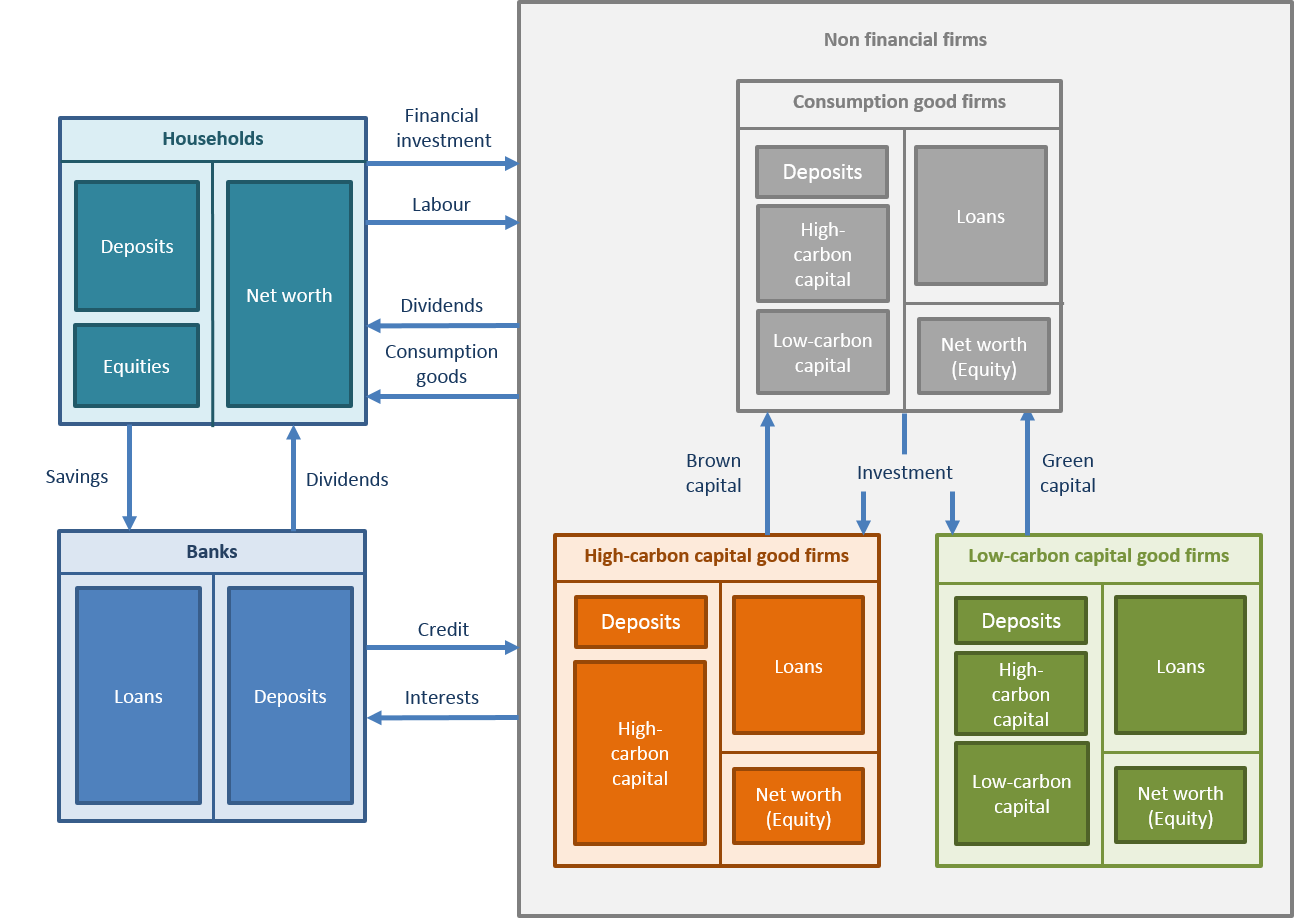
\includegraphics[width=12cm]{Figures/ModelOverview.png}
\label{fig:Model}
\end{figure}

The aim of the paper is to study how a misalignment between market expectations and the transition to low-carbon capital stock may lead to unexpected and potentially detrimental financial dynamics. For this purpose we develop a macroeconomic model with five distinct sectors:
\begin{enumerate}[noitemsep,nolistsep,leftmargin=*]
\item \emph{Households}\footnote{As will be shown in Section \ref{sec:model}, we further disaggregate households into two distinct sectors for analytical purposes: wage-earners and financial investors. However, these sectors conceptually represent two functions both performed by the same household sector, and are thus presented together here.}.
We assume households to perform three main economic activities: supply labour, consume, and invest in financial assets. Households' income is given by the sum of wages, dividends and capital gains. In each period they decide their consumption level depending on their expected disposable income and their wealth. There are four types of assets households can invest their savings in: cash, equities of consumption good firms, equities of traditional capital good firms and equities of low-carbon capital good firms. Households' financial wealth is thus the sum of cash and equities of the three productive sectors they hold. 
\item \emph{Consumption good firms}. Firms producing the single consumption good employ labour and physical capital - both high- and low-carbon - in order to satisfy the aggregate demand for consumption goods coming from households. The price of the consumption good is set by imposing a mark-up on production unit costs.
\item \emph{High-carbon capital good firms}. Firms producing the traditional, high-carbon capital good employ labour and physical capital - only of the high-carbon kind - to satisfy the demand for traditional capital coming from consumption good firms, low-carbon capital good firms and from inside the sector. 
\item \emph{Low-carbon capital good firms}. Firms producing the low-carbon capital good employ labour and physical capital - both low- and, for the first periods of its existence, high-carbon - to satisfy the demand for low-carbon capital coming from consumption good firms and from inside the sector. 
\item \emph{Banks}. The banking sector in our model has the double role of holding deposit accounts for households and creating credit for non-financial firms. We assume banks to accommodate the entire demand for loans, but to discriminate among sectors by applying a different interest rate depending on the perceived risk of the sectors to which they are lending, in turn a function of their return rate. Interests are then transferred to households as dividend payments. Given that there is no government or central bank in this model, private banks create the entire money supply circulating in the economy. \\
\end{enumerate}

As can be appreciated in Figure \ref{fig:Model}, which gives a schematic overview of the model, we make extensive use of double-entry accounting depicting each sector as a set of interacting assets and liabilities, in line with Stock-Flow Consistent (SFC) macroeconomic modelling methods \citep{Caverzasi2015, Godley:2007}. SFC models are consistent in that every monetary flow is recorded as a payment for one sector and a receipt for another sector, and every financial stock is recorded as an asset for a sector and a liability for another sector. For instance, deposits are an asset for households and firms while being a liability for the banking system. 

In each period all productive sectors decide how much to invest in the way described in section \ref{sec:inv}. They then have to decide how to allocate their investment demand across the two capital goods. We assume the productivity of the two capital types to be identical; i.e. they are equally effective at producing the consumption good. However, their price is different. We make a counterfactual assumption about prices, in order to abstract from the market and policy reasons why the transition might or might not happen. Specifically, we assume that the price of the low-carbon capital good is lower than the price of the traditional capital good. The aim of this work is  to study how, even when abstracting away from issues related to the economic convenience of clean technologies, financial market sentiments and expectations might still have deep effects on the speed, smoothness or even the realisation of the low-carbon transition. In other words, we do not focus here on \emph{why} or \emph{how} the transition takes place\footnote{This will be be addressed in a forthcoming companion article}; we instead assume that all economic conditions are satisfied for firms to be interested in purchasing low-carbon capital goods and explore whether and how even in these conditions financial dynamics might put the transition at peril.

Our  theoretical structure is similar to \citet{Caiani2014}, who develop a Schumpeterian two-sector model to investigate the economic and financial implications of the emergence of an innovative sector. In particular, we adopt a similar representation of the financial market, in which firms have emitted equities, and financial investors allocate their wealth across the equities of the different sectors according to two factors: 1. a `trend' term, which depends on the relative market share of each sector; 2. a `fluctuation' term that depends on relative financial returns (see Section \ref{sec:port}). 

In order to study the role of market sentiments, however, we introduce the possibility for investors to form expectations and allow them to be influenced by irrational behaviour and imperfect knowledge. More specifically, we assume that in each period financial investors form expectations around the future growth rate of the high-carbon and low-carbon capital stocks. Expectations here are adaptive, in that they are formed by looking at the recent past trend in capital dynamics and projecting the same trend into the near future. However, as argued in Section \ref{sec:intro}, financial investors may also display an `irrational' bias in favour of the well-known traditional high-carbon capital sector and away from the untested low-carbon technology. This would lead them to over-optimistically estimate the relative growth of the high-carbon capital sector and thus allocate a higher-proportion of their financial wealth into high-carbon equities. This `irrational climate apathy' is represented in the model by parameter $\theta$. 

Additionally, we assume financial investors to base their decision on limited private information and imperfect knowledge \citep{Daniel1998}, as they are not fully able to observe capital stocks dynamics. This applies to all capital stocks, not just low-carbon stocks, and may be due to scarce or conflicting data, confirmation bias, filtering information to manage complexity, reliance on peer networks, or other reasons. As a consequence, in aggregate we expect financial investors to adapt their expectations moving from the previously expected capital values towards the actual ones, but only to a certain extent. This `blindness', which creates a wedge between actual and perceived capital stocks, is represented in the model by parameter $\phi$.


%%%%%%%%%%%%%%%%%%
%%%%%%%%%%%%%%%%%%
\section{The model}
\label{sec:model}
%%%%%%%%%%%%%%%%%%
%%%%%%%%%%%%%%%%%%

We consider a closed economy in discrete time. Three goods exist in the economy: a consumption good ($y_c$), a high-carbon investment good ($y_h$) and a `low-carbon' investment good ($y_l$). Six sectors populate the economy: wage-earners, financial investors\footnote{As mentioned in Section \ref{sec:concept}, wage-earners and financial investors can be thought as representing two function of the same household sector. We distinguish them here for analytical clarity.}, firms producing the consumption good, firms producing the high-carbon investment good, firms producing the low-carbon investment good, and private banks. 

For the remainder of the paper we will use upper-case letters to denote nominal variables and lower-case letters to denote real variables\footnote{For instance, $Y_C$ represents the monetary value of the consumption sector output, while $y_c$ represents the quantity of consumption goods produced.} We simplify time notation by assuming all variables to be at time $t$, unless explicitly specified. We also simplify exposition when possible by using $x$ to indicate the three productive sectors; that is, $x=c,h,l$.

On top of climate-related expectations, explained in detail in Section \ref{sec:exp}, we assume households and firms to form expectations around the development of some relevant macroeconomic variables (e.g. income, profits, dividends, capital gains). We assume the expected value of a variable to be a function of its recent past dynamics, corrected by a term proportional to the accuracy of past expectations\footnote{As an example, expected nominal profits $F_x$ in sector $x$ are equal to:
$F_x^e = \left(1 + \eta\hat{F}_x\right)\bar{F}_x + \nu\left(F_{x,-1} - F^e_{x,-1}\right) \label{eq:expect}$
where $\hat{F}_x$ indicates the growth rate of profits in the previous period and $\bar{F}_x$ represents the average of profits over the previous four periods.}.

For reasons of space and clarity, we here opt for presenting only the most relevant analytical parts of the model. A full description of the model, comprehensive of all equations and relative code, is available as an online appendix\footnote{The code of the model is also avilable at https://github.com/greenmacro/strandedassets}.


%%%%%%%%%%%%%%%%%%
\subsection{Production}
\label{sec:output}
%%%%%%%%%%%%%%%%%%

Sectoral output is given by the demand for the specific good that the sector produces. That is, production of the consumption good $y_c$ is determined by consumption demand by households, while production of both investment goods $y_h$ and $y_l$ is given by investment demands by firms.
\begin{align}
y_c&=c,  \\
y_h&=i_{h,c}+i_{h,h}+i_{h,l}, \\
y_l&=i_{l,c}+i_{l,l},
\end{align}
where $i_{\alpha,\beta}$ indicates investment of sector $\beta$ in good $\alpha$. For instance, $i_{l,c}$ refers to the investment in low-carbon capital carried out by firms in the consumption good sector. 

Firms produce output using a combination of capital stock ($k_h$ or $k_l$) and labour ($n$). Demand defines the sectoral demand for input factors, thus determining both employment levels and rates of capacity utilisation. Employment $n_x$ in sector $x$ is given by sectoral output divided by sectoral labour productivity $\xi_{n,x}$, while aggregate employment is the sum of employment in each sector. The employment rate $\gamma$ is calculated as total employment divided by labor force $lf$, whose value is exogenous.
\begin{align}
n_x&=\dfrac{y_x}{\xi_{n,x}}, \\
n_{tot} &= n_c + n_i + n_k, \\
\gamma&=\dfrac{n_{tot}}{lf}.
\end{align}

Similarly, capital utilisation $u_x$ in sector $x$ is the ratio between the capital stock actually employed to satisfy demand $y_x$ and the available capital stock. This is equivalent to the ratio between actual and potential output. Defining the latter as the output producible using the whole amount of physical capital available, capacity utilisation rate $u_x$ can be written as:
\begin{gather}
u_x = \frac{y_x}{\xi_{h} k_{h,x} + \xi_{l} k_{l,x}},
\end{gather}
where $\xi_{h}$ and $\xi_{l}$ are the productivity of high-carbon and low-carbon capital, respectively, which we assume to identical across sectors (i.e. each type of capital is equally productive at producing all types of goods). 

%%%%%%%%%%%%%%%%%%
\subsection{Income and consumption}
\label{sec:income}
%%%%%%%%%%%%%%%%%%

In every period households consume a proportion $\alpha_1$ of their expected real disposable income $yd^e$ and a proportion $\alpha_2$ of their previous period real wealth\footnote{We assume different propensities to consume depending on the type of income (i.e. capital vs. labor) and on the type of wealth (i.e. money holding vs. financial wealth).}. We follow \citet{Godley:2007} in defining real expected disposable income as the difference between real expected income and the loss of real wealth due to inflation.
\begin{align}
c&=\alpha_1 yd^e + \alpha_2 v_{-1},\\
yd^e&=\dfrac{YD^e}{p_c}-\pi_c \dfrac{V_{-1}}{p_c}.
\end{align}

Nominal disposable income of wage-earners $YD_w$ is given by the sum of sectoral wage bills (equal to the wage rate $W_x$ times the number of people employed $n_x$)
\begin{align}
YD_w=W_c n_c+ W_h n_h+W_l n_l.
\end{align}

Nominal disposable income of investors is the sum of dividends coming from productive sectors ($FD_x$) and banks ($FD_b$):
\begin{align}
YD_f=FD_c+FD_h+FD_l+FD_b.
\end{align}

Whatever proportion of income is not consumed, is saved and thus contributes to the accumulation of financial wealth. While wage-earners allocate their entire financial wealth $V_w$ in cash, financial investors also have the option of investing their financial wealth $V_f$ into the equities of the three productive sectors. Their financial wealth is thus given by: 
\begin{align}
V_w&=M_w, \\
V_f&=M_f+e_cp_{c,e}+e_hp_{h,e}+e_lp_{l,e},
\end{align}
where $M_w$ and $M_f$ represent cash holdings of wage-earners and financial investors, respectively.

%%%%%%%%%%%%%%%%%%
\subsection{Investment in physical capital}
\label{sec:inv}
%%%%%%%%%%%%%%%%%%

We follow \citet{Fazzari1986} and \citet{Caiani2014} in assuming that all productive sectors choose their desired rate of growth of capital $g_{x}$, according to three factors. First, capital growth is positively related to expected capacity utilization $u_x^e$. defined as the ratio of expected output ($y_x^e$) over full capacity output. Rising expected utilization is an indication to firms that existing capacity is insufficient to meet future demand, threatening missed orders and loss of market share. It is also a proxy for anticipated excess profits, which can be put toward expanded capacity. Second, desired capital growth is assumed to be depressed when the cost of capital is high or when the sector is already highly leveraged, reflected in a negative `banking' factor made of the real interest rate $rr_{x}$ - defined as the nominal interest rate $r_{l,x}$ deflated by capital price inflation $\pi_k$ - and the leverage level $\lambda_x$ - defined as the ratio of outstanding loans to the replacement of value of the capital stock at current prices. Third, capital expansion is stimulated by market valuation as measured by Tobin's q, $q_x$, defined as the ratio between the market value of equity – the number of shares multiplied by their price – and its book value – calculated as the difference between assets and liabilities \citep{Tobin1969}. When $q$ is equal to 1 the equities of the sector are valued so that their total market value is equal to the underlying net capital stocks measured at book value. A sectoral $q$ higher than 1 indicates instead that financial markets value the equities of the sector more than the book value of their net capital stock; this would make it easier for the firm to raise finance on the market and make physical investment relatively more convenient. In our model, the book value of sectoral equity is given by the physical capital stocks $k_{h,x}$ and $k_{l,x}$, valued at their respective prices $p_h$ and $p_l$, less the stock of loans $L_x$.
\begin{align}
g_{x}&=\eta_{0} + \eta_{1} u_x^e-\eta_{2} rr_{l,x} \lambda_{x,-1}+\eta_3 q_{x,-1}, \label{eq:gx}\\
u_x^e&=\dfrac{y_x^e}{k_{h, x,-1}\xi_h+k_{l, x,-1}\xi_l},\\
rr_x&=\dfrac{1+r_x}{1+\pi_k}-1,\\
\lambda_x&=\dfrac{L_x}{p_hk_{h,x}. +p_l.k_{l,x}},\\
q_x&=\dfrac{e_x.p_{x,e}}{k_{h,x}.p_h+k_{l,x}.p_l-L_x}.
\end{align}

Total real gross investment takes into account both desired growth in capacity and depreciation, setting the floor for investment to zero (i.e. firms are not allowed to disinvest):
\begin{align}
i_x = \max\left(g_x y_{x,-1} + \delta_h k_h + \delta_l k_l,0\right).
\end{align}

While both capital good producing sectors employ exclusively their own type of capital (with the exception of low-carbon firms that are forced to use high-carbon capital in the initial period of their existence due to lack of sufficient low-carbon capital), firms producing the consumption good have the option of choosing between low-carbon and high-carbon capital. In order to decide between the two, consumption good firms compare the total unit costs of each capital good $UC_{h,c}$ and $UC_{l,c}$ to see which is the most convenient. Total unit costs are composed of variable unit costs - in our model these are only labor costs - and fixed unit amortization costs, assumed to be linear over the life time of capital $\delta_x$.
\begin{align}
UC_{h,c} &= \dfrac{W_c}{\xi_h \ell_h} + \dfrac{p_h}{\delta_h \xi_h},\\
UC_{l,c} &= \dfrac{W_c}{\xi_l \ell_l} + \dfrac{p_l}{\delta_l \xi_l},
\end{align}
where $\ell_h$ and $\ell_l$ represent the the capital-labour ratio of sector $h$ and $l$, respectively. We assume investment to be irreversible, so that capital stocks disappear from the model only through depreciation (i.e., high-carbon capital cannot be transformed into low-carbon capital, and viceversa)

We assume sectoral unit costs to affect the relative preferences of consumption good firms. More specifically, we compute the proportion $\beta$ of total investment of the consumption good sector $i_c$ directed towards low-carbon capital goods as a function of the difference between sectoral unit costs. Since the allocation between high- and low-carbon capital investment ($i_{h,c}$ and $i_{l,c}$) is done on the basis of sectoral output we adjust the capital investment values using capital productivities:
\begin{align}
i_{l,c} &= \beta \dfrac{i_c}{\xi_l},\\
i_{h,c} &= (1-\beta) \dfrac{i_c}{\xi_h},\\
\beta &= \dfrac{1}{1+\beta_0 e^{\beta_1 \Delta UC}},\quad \Delta UC \equiv UC_{l,c}-UC_{h,c}.
\end{align}

In the limit that the unit cost of operating low-carbon capital is much larger than that for high-carbon capital, we expect very little investment in low-carbon capital, so $\beta$ should approach zero. Taking the contrary case of a high unit cost of operating high-carbon capital, $\beta$ should approach one. The specification for $\beta$ above displays this behavior. When unit costs are equal in the brown and green sector, $\beta = 1/(1 + \beta_0)$. If $\beta_0 > 1$, the share of green capital is less than that of brown capital at equal unit costs, whereas if $\beta_0 < 1$ the share of green capital is greater than that of brown capital. The parameter $\beta_0$ thus reflects a bias toward low- or high-carbon capital. The parameter $\beta_1$ represent the strength of the cost factor in firms' investment decisions.



%%%%%%%%%%%%%%%%%
\subsection{Financing}
\label{sec:port}
%%%%%%%%%%%%%%%%%%
Total nominal investment $I_x$ in sector $x$ is equal to real investment in each type of capital ($i_{h,x}$ and $i_{l,x}$) multiplied by its price:
\begin{align}
I_x = p_h i_{h,x} + p_l i_{l,x}.
\end{align}

Firms finance new investment through retained earnings and loans, through the following decision process. First, firms decide on desired dividend payout based on a target nominal return rate $R_x^T$, expected nominal capital gains $CG_x^e$, and previous-period equity price, $p_{x,-1}^e$, with a fixed quantity of shares $e_x$,
\begin{gather}
FD_x^T = R_x^T e_x p_{x,-1}^e - CG_x^e,
\end{gather}
where capital gains $CG_x$ are in turn equal to the variation of equity price $p_{x,e}$ during the last period multiplied by the total number of shares $e_x$\footnote{We assume the total number of shares to be constant for the two original sectors and to be constant after the initial issuance due the low-carbon sector IPO.}:
\begin{align}
CG_x&= e_x \Delta p_{x,e}.
\end{align} 

They then determine desired retained earnings $RE_x^T$ based on their investment decision $I_x$, target leverage ratio $\lambda_x^T$, previous-period level of loans $L_{x,-1}$ and current-period nominal capital stock $K_x$,
\begin{gather}
RE_x^T = L_{x,-1} + I_x - \lambda_x^T K_x.
\end{gather}
If profits are sufficient to cover the sum of desired retained earnings and dividends, firms deposit the remainder, increasing their money buffer stock $M_x$. If profits are insufficient, they use the money they have saved to meet their targets; if that is still insufficient, they ration both dividends and retained earnings in proportion to their desired levels.

Net addition to loans is the difference between firms' investment decision and retained earnings.
We assume banks to accommodate any demand for loans coming from productive sectors, but to discriminate among them by setting the interest rate on loans ($r_{l,x}$) as a mark-up on the policy rate ($r_l$) where the mark-up depends on the perceived risk of the sector. We calculate the latter as a function of the difference between the average historical return rate of the sector net of interest ($\bar{r}_x$) and an exogenously determined benchmark return rate ($r_b$).
\begin{align}
r_{l,x} &= r_l\left[1 + \frac{1}{1 + e^{\kappa(r_x^a - r_b)}} \right], \\
\bar{r}_x&=\frac{1}{4}\sum_{n=1}^{4}\frac{F_{x,-n}-r_{l,x,-n}L_{x,-(n+1)}}{p_{h,-(n+1)}k_{h,x,-(n+1)}+p_{l,-(n+1)} k_{l,x,-(n+1)}}.
\end{align}

%%%%%%%%%%%%%%%%%%
\subsection{Portfolio allocation}
\label{sec:port}
%%%%%%%%%%%%%%%%%%

We follow \citet{Brainard1968} in assuming that financial investors allocate their expected financial wealth $V^e_{f}$ among the equities in the three sectors ($e_c$, $e_h$ and $e_l$) and money held for financial purposes ($M_f$) in the following way:
\begin{equation}
\left(
\begin{matrix} M_f \\ p_{c,e}e_c \\ p_{h,e}e_h \\ p_{l,e}e_l \end{matrix}
\right)
=\left(
\begin{matrix}
	\lambda_{10} && \lambda_{11} && \lambda_{12} && \lambda_{13} && \lambda_{14} \\
	\lambda_{20} && \lambda_{21} && \lambda_{22} && \lambda_{23} && \lambda_{24} \\
	\lambda_{30} && \lambda_{31} && \lambda_{32} && \lambda_{33} && \lambda_{34} \\
	\lambda_{40} && \lambda_{41} && \lambda_{42} && \lambda_{43} && \lambda_{44}
\end{matrix}
\right)
\left(
\begin{matrix} 1 \\ \text{R}_m \\ \text{R}_c \\ \text{R}_h \\ \text{R}_l \end{matrix}
\right) V^e_{fc}.
\label{eq:portfolio}
\end{equation}

Real returns of financial assets are equal to:
\begin{align}
\text{R}_m &= \frac{1}{M}\left(\frac{M}{1+\pi_c} - M\right) = \frac{-\pi_c}{1 + \pi_c} \label{eq:Rm} \\
\text{R}_x &= \chi_\text{div}\left(\frac{1 + r_x^e}{1 + \pi_c} - 1\right) \nonumber\\
			 &\quad + \chi_\text{prof}\left(\frac{1 + rg_x^e}{1 + \pi_c} - 1\right) \nonumber\\
			 &\quad + \chi_\text{gains}\left(\frac{1 + cg_x^e}{1 + \pi_c} - 1\right), \label{eq:Rx}
\end{align}
where $cg_x^e$ are expected real capital gains, $r_x^e$ expected real dividends and $rg^e_x$ expected real profits, all computed relative to the sector market capitalisation in the previous period, and $\pi_c$ is the inflation rate for consumption goods.

Following \citet{Godley:2007} and \citet{Caiani2014}, we impose some conditions on the $\lambda^a_{mn}$ coefficients. The equality between expected wealth and allocation is ensured by requiring
\begin{gather}
\sum_{m=1}^4 \lambda_{m0} = 1,\\
\sum_{m=1}^4 \lambda_{mn} = 0,\> n\in\{1,\ldots,4\}, \\
\lambda_{mn} = \lambda_{nm},\> m,n\in\{1,\ldots,4\}. \label{eq:simm}
\end{gather}

Equation \ref{eq:simm} imposes a symmetry condition that ensures the effect on holdings of asset $n$ due to a change in the real rate of return of asset $m$ is equal to the effect on holdings of asset $m$ due to a change in the real rate of return of asset $n$.
			
We follow \citet{Tobin1969} in assuming that, in the long run, Tobin's $q$ should be equal to 1; i.e. in each sector the value of equity should be equal to the market value of the capital stock less the amount of loans. Hence we interpret the vector of $\lambda_{m0}$ as the long-run positions of the sectors and set them equal to the expected capital stock sectoral shares (see Section \ref{sec:exp}). In the short-term, however, financial positions can substantially deviate from their equilibrium values due to relative return rates (Equations \ref{eq:Rm} and \ref{eq:Rx}), introducing fluctuations in the model. In other words, investors allocate their expected wealth according to: 1. a long-run term that depends on the expected share of capital of each sector; 2. a short-run term that depends on sectoral relative returns. 


%%%%%%%%%%%%%%%%%%
\subsection{Climate market sentiments}
\label{sec:exp}
%%%%%%%%%%%%%%%%%%

The computation of the long-term factors in portfolio sectoral allocation choices $\lambda_{m0}$ is where we introduce cognitive biases and market sentiments around the likelihood of a low-carbon transition. 

As argued in Section \ref{sec:intro}, we assume financial investors to suffer from an inherent bias in favor of the high-carbon capital sector that leads them to redistribute a proportion of the expected overall capital growth from the low-carbon to the high-carbon sector. Therefore investors form expectations around the future growth of the sectors looking at past sectoral capital growth, but correct them according to an `irrational climate apathy' parameter $\theta\in[0,1]$ while keeping the overall expected growth of both capital sectors $\hat{k}$ constant and in line with observed values. We assume investors to hold unbiased expectations around the growth of capital stocks in the consumption sectors. 

\begin{align}
\hat{k}_{l,l}^e &= (1-\theta) \dfrac{\hat{k} - \sigma_{h,h} \hat{k}_{h,h} - \sigma_{h,l} \hat{k}_{h,l}}{1-\sigma_{h,h}- \sigma_{h,l}}, \label{eq:klle}\\
\hat{k}_{h,h}^e &= \dfrac{\hat{k}-(1- \sigma_{h,h}-\sigma_{h,l}) \hat{k}^e_{l,l} - \sigma_{h,l}\hat{k}_{h,l}}{\sigma_{h,h}}, \label{eq:khhe}\\
\hat{k}_{h,l}^e &= \dfrac{\hat{k}-(1- \sigma_{h,h}-\sigma_{h,l}) \hat{k}^e_{l,l} - \sigma_{h,h}\hat{k}_{h,h}}{\sigma_{h,l}}, \label{eq:khle}\\
\hat{k}_{h,c}^e &= \hat{k}_{h,c}, \label{eq:khce}\\
\hat{k}_{l,c}^e &= \hat{k}_{l,c}, \label{eq:klce}
\end{align}
where $\sigma_{h,h} = \frac{k_{h,h}}{k_{h,h} + k_{h,l} + k_{l,l}}$ and $\sigma_{h,l} = \frac{k_{h,l}}{k_{h,h} + k_{h,l} + k_{l,l}}$ are relative capital shares. Higher values of $\theta$ indicate that financial investors exhibit a stronger disbelief in the capacity of the low-carbon capital sector to expand, and transfer a larger proportion of the `unbiased' low-carbon growth expectations towards the high-carbon sector. We further smooth expectations by taking the four-period average of expected growth rates as calculated in Equations (\ref{eq:klle}) to (\ref{eq:klce}) to find the expected levels of capital stocks $k_{l,l}^e$, $k_{h,h}^e$, $k_{h,l}^e$, $k_{h,c}^e$ and $k_{l,c}^e$.

In the following period, once financial wealth has been allocated and physical investment performed,  all the relevant capital stock variables will display updated values. Given uncertainty and cognitive biases, we expect some gap to exist between the actual values and the previous-period expected values. We here assume investors to suffer from an additional form of myopic behaviour, in that they are able to adjust their perceptions towards the actual levels only to a limited extent, which we measure through a `blindness' or `expectations stickiness' parameter $\phi\in[0,1]$. For simplicity, we assume this myopia to be relevant only in the capital goods sectors. 

\begin{align}
k_{l,l}^{Perc} &=  (1-\phi) k_{l,l} + \phi k_{l,l,-1}^e,\\
k_{h,h}^{Perc} &=  (1-\phi) k_{h,h} + \phi k_{h,h,-1}^e,\\
k_{h,l}^{Perc} &=  (1-\phi) k_{h,l} + \phi k_{h,l,-1}^e,\\
k_{h,c}^{Perc} &=  k_{h,c},\\
k_{l,c}^{Perc} &=  k_{l,c},
\end{align}
where the $Perc$ superscript indicate `perceived' values. Higher values of $\phi$ indicate that expectations of financial investors are sticky and adapt towards the actual values only to a small extent; or, alternatively, that there is little information circulating among investors about the actual development of the capital sectors. 

The final step of the process is to get to a definition for the set of $\lambda_{m0}$. We assume these to be a function of the expected present value of sectoral capital stocks, computed using both the \emph{perceived} capital stock levels and the {expected} sectoral growth rates.From the investor's perspective, the present value is given by a discounted sum of expected growth over the lifetime $T$ of the perceived level of capital stock, reduced by the firm's target leverage $\lambda_x^T$. Using the policy rate ($r_l$) as the the discount rate, the present value for a generic stock, $k$, is given by
\begin{gather}
k^{PV} = (1 - \lambda^T) k^{Perc} \sum_{t = 0}^{T - 1}\zeta^t,\quad\zeta \equiv \frac{1+\hat{k}^e}{1+r_l}.
\end{gather}
The present value is
\begin{gather}
k^{PV} = (1 - \lambda^T) k^{Perc} \frac{1 - \zeta^T}{1 - \zeta}.
\end{gather}
For each sector, we sum over high- and low-carbon capital, so
\begin{align}
k_{c}^{PV} &= (1 - \lambda_c^T) \left(k_{h,c}^{Perc} \dfrac{1-\zeta_{h,c}^T}{1-\zeta_{h,c}} + k_{l,c}^{Perc} \dfrac{1-\zeta_{l,c}^T}{1-\zeta_{l,c}}\right),\\
k_{h}^{PV} &= (1 - \lambda_h^T) k_{h,h}^{Perc} \dfrac{1-\zeta_{h,h}^T}{1-\zeta_{h,h}},\\
k_{l}^{PV} &= (1 - \lambda_l^T) \left(k_{l,l}^{Perc} \dfrac{1-\zeta_{l,l}^T}{1-\zeta_{l,l}} + k_{h,l}^{Perc} \dfrac{1-\zeta_{h,l}^T}{1-\zeta_{h,l}}\right),
\end{align}
where
\begin{gather}
\zeta_{i,j} = \frac{1+\hat{k}^e_{i,j}}{1+r_l},\:i,j=c,h,l.
\end{gather}

The $\lambda_{m0}$ are then computed in terms of these expected income streams. The long run position for money, $\lambda_{10}$, is an exogenous parameter. Otherwise,
\begin{gather}
\lambda_{m0} = (1 - \lambda_{10}) \frac{k_m^{PV}}{\sum_{n=2}^4 k_n^{PV}}, \quad x=c,h,l.
\end{gather}

%%%%%%%%%%%%%%%%%%
%%%%%%%%%%%%%%%%%%
\section{Numerical simulations}
\label{sec:sim}
%%%%%%%%%%%%%%%%%%
%%%%%%%%%%%%%%%%%%

The model is simulated using R\footnote{The source code of the model is available in the Appendix and at https://github.com/greenmacro/strandedassets. We also make use of the PKSFC package, available at https://github.com/s120/pksfc.}. For simplicity and easiness of computation, we assume the model to start from a stationary state in which the low-carbon sector is still to be created. Both the consumption and the high-carbon capital sector employ only high-carbon capital to produce. At time 20, we assume the low-carbon sector to enter the capital goods market. At first, the low-carbon sector is funded through loans and, since the stock of low-carbon capital available is still insufficient, it employs high-carbon capital in its production process. Then, at time 40, we assume the low-carbon sector to start issuing equities enter the financial market through an IPO (Initial Public Offering).

As argued in Section \ref{sec:concept}, we here assume assume the two capital stocks $k_h$ and $k_l$ to be identical in many ways - for instance, they are equally efficient in producing output ($\xi_h=\xi_l$), display the same capital-labor ratio ($\ell_h=\ell_l$) and have the same depreciation rate ($\delta_H=\delta_l$) - but to differ in their price. In particular, we assume that the price of high-carbon capital is higher than the price of the low-carbon capital. This allows us to concentrate on the effects of financial sentiments on the transition, irrespective of whether this `naturally' takes place and why.

To study the results of the numerical simulations, we first show the long-run dynamics of the model with `unbiased' market sentiments. We then focus the analysis on the role of climate financial sentiments along the low-carbon transition in Section \ref{sec:SensAnal}. 


%%%%%%%%%%%%%%%%%%
\subsection{Baseline scenario}
\label{sec:BAUsim}
%%%%%%%%%%%%%%%%%%

\begin{figure} %float with two figures
\centering
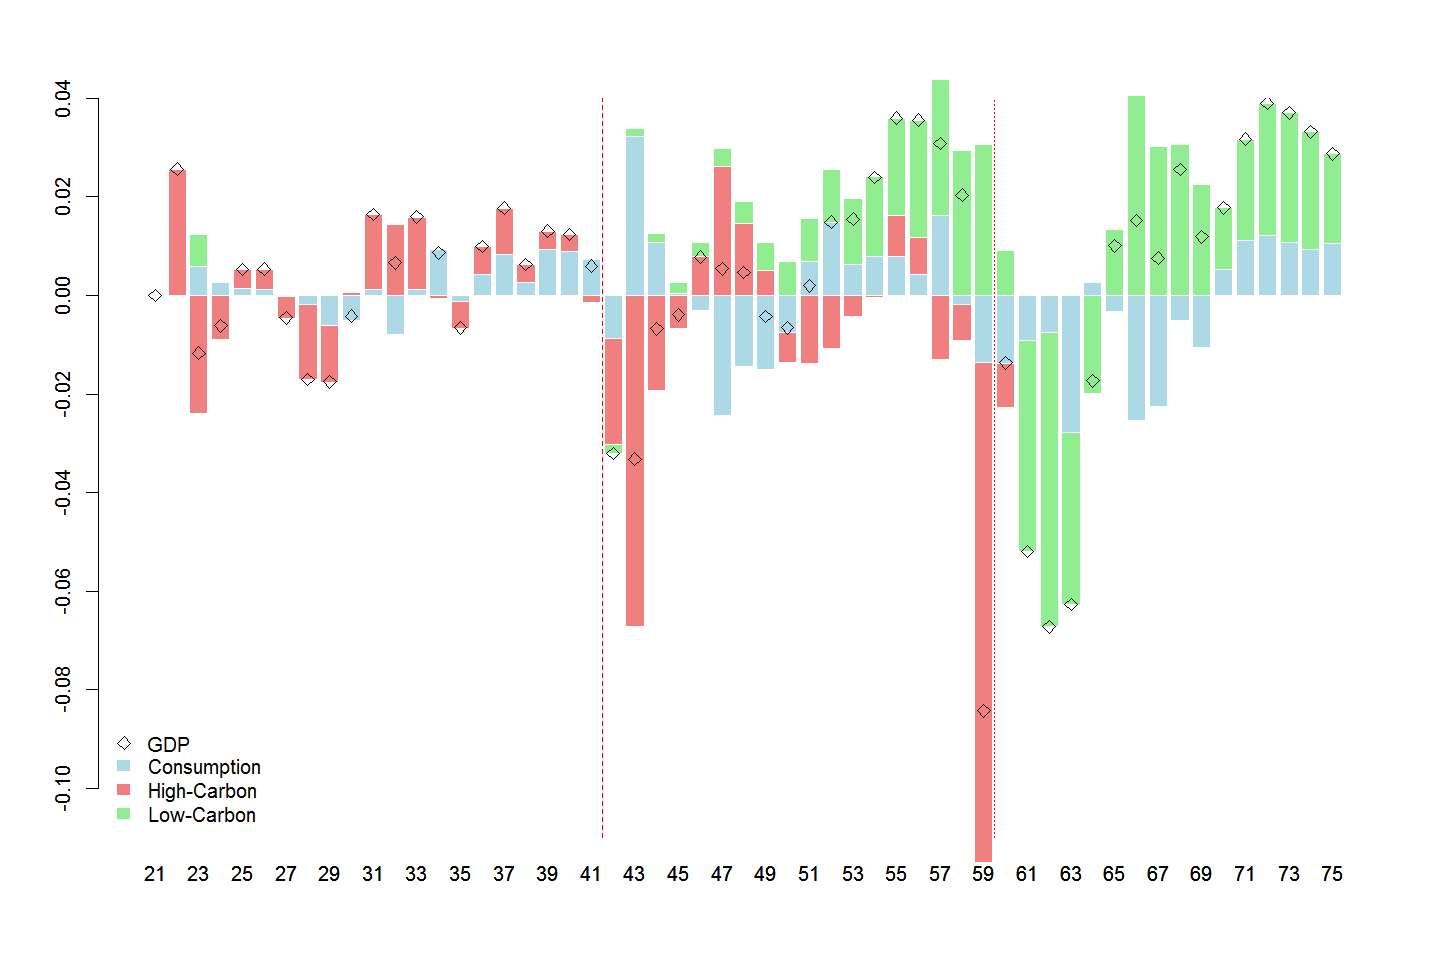
\includegraphics[width=\linewidth]{Figures/baselineGDP.png}
\caption{Change in sector output as \% of GDP - Baseline scenario} 
\label{fig:BaselineGDP}
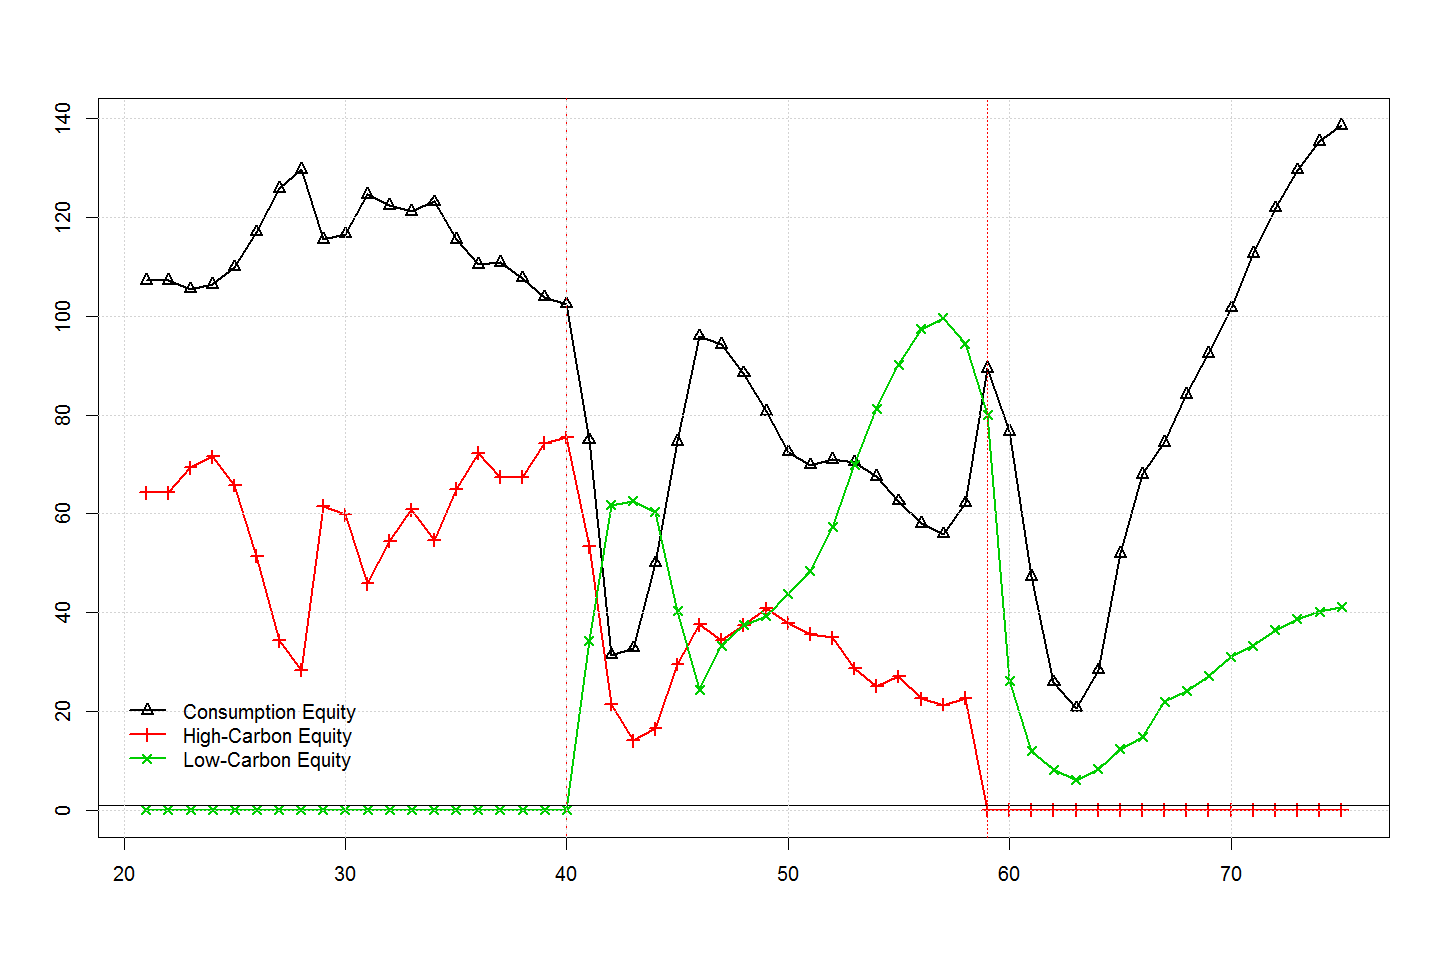
\includegraphics[width=\linewidth]{Figures/baselineEquityPrice.png}
\caption{Sectoral equity prices - Baseline scenario}
\label{fig:BaseEqPrice}
\end{figure}
In the start-up phase of the low-carbon sector, it requires high-carbon capital initially. The immediate reaction to the entrance of the low-carbon sector is thus an increase in output driven by demand for high-carbon capital from the new sector (see Figure \ref{fig:BaselineGDP}). The price of high-carbon capital falls slightly, despite increases in employment and capacity utilization, because firms adjust prices to meet a target return rate on capital. Lower inflation then leads to an increase in the real interest rate, which negatively affects investment decisions in the consumption good sector. This cascade of effects leads to a short-lived slump around period 30. After that, all sectors expand due to increased employment in the capital good sectors and a general improvement of financial conditions as measured by Tobin’s $q$.

In period 40, the low-carbon sector launches its IPO, strongly impacting the equities of both  the consumption and the high-carbon sectors as financial wealth is partly reallocated towards the new sector (see Figure \ref{fig:BaseEqPrice}). Since Tobin's $q$ is one of the determinants of sectoral investment function (Equation \ref{eq:gx}), the decrease of equity value of the sectors drives a reduction in physical investment. In the high-carbon sector, this negative effect is exacerbated by falling demand from the consumption sector, due to both a general slump and substitution of low-carbon for high-carbon capital in new investment. Investors shift out of the high-carbon sector, reducing its market capitalization, while falling profits drive the high-carbon sector to bankruptcy in period 59.

The exit of the high-carbon sector from the market leads to a loss of wealth, both from a fall in the market price of equities and the banks' writing off loans to the high-carbon sector. It also leads to a loss of wage income. These effects trigger a strong real and financial crisis for the remaining two sectors, with declining output and a drop in equity values. In a reverse of the processes following the introduction of the low-carbon sector, low capital utilization combined with target-return pricing stimulates inflation, driving down real interest rates. The low interest rates stimulate the low-carbon and consumption sectors after a few periods of recession. As investors shift from money toward equities, they drive Tobin's $q$ higher, stimulating further investment.

%%%%%%%%%%%%%%%%%%
\subsection{Playing with market sentiments}
\label{sec:SensAnal}
%%%%%%%%%%%%%%%%%%

\begin{figure}[h!]
\begin{minipage}[b]{.5\linewidth}
\centering\large  
  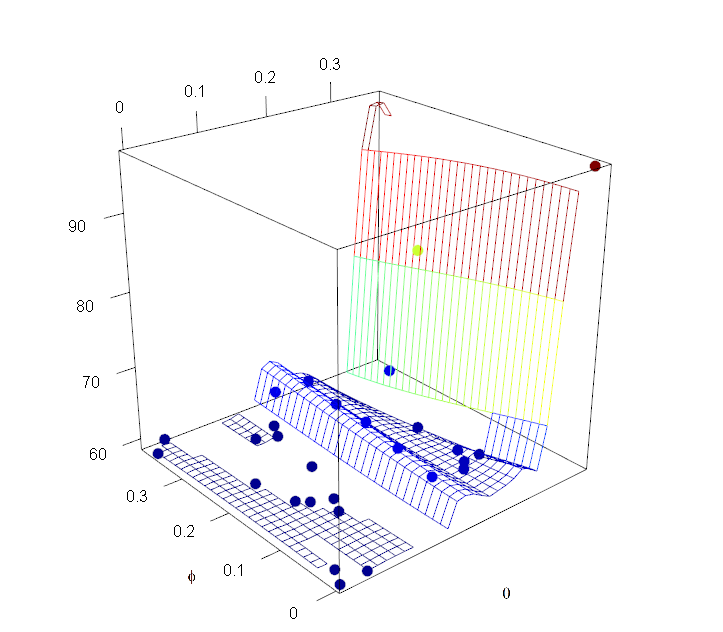
\includegraphics[width=7cm]{Figures/SensExitPeriod.png}
  \subcaption{High-carbon sector exit period}\label{Fig:SensExitPeriod}
\end{minipage}
\quad \quad
\begin{minipage}[b]{.5\linewidth}
\centering\large 
    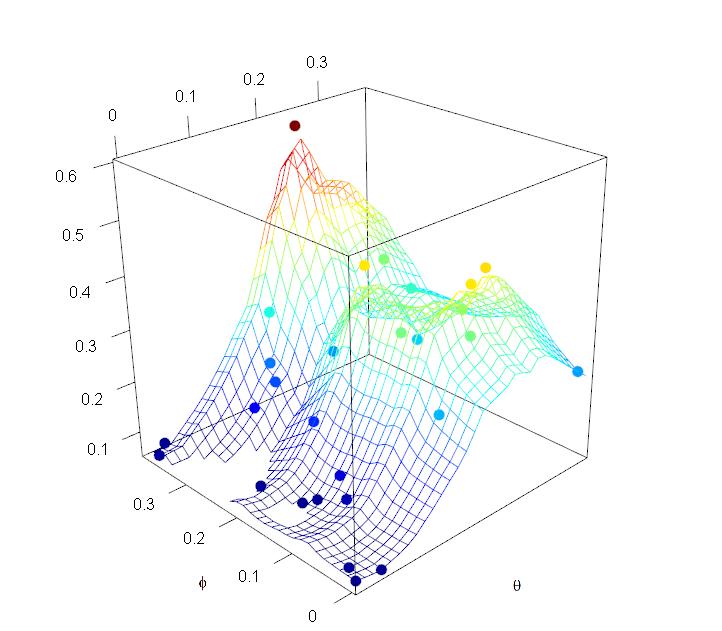
\includegraphics[width=7cm]{Figures/SensOutputVolatility.png}
    \subcaption{Output volatility index}\label{Fig:SensOutputVol}
\end{minipage}
\vspace{0.2cm}
    \begin{minipage}[b]{.5\linewidth}
\centering\large 
    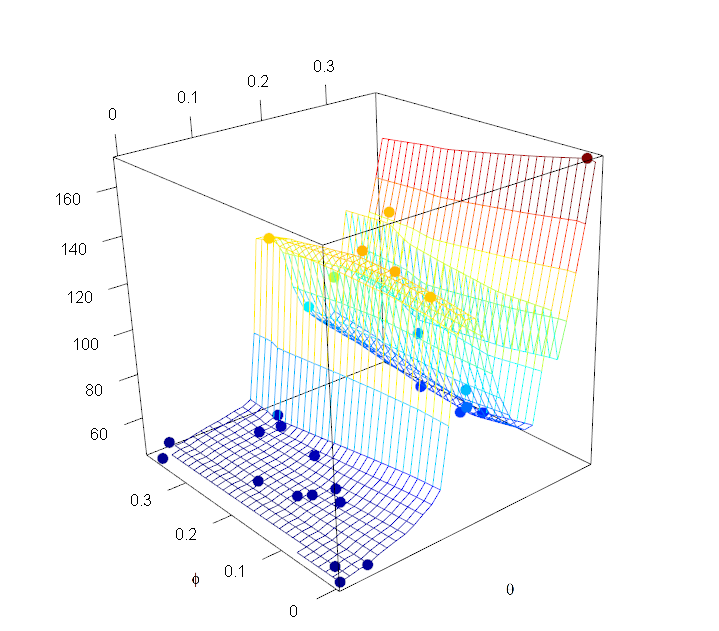
\includegraphics[width=7cm]{Figures/SensPhysicalStranded.png}
    \subcaption{Physical stranded assets}\label{Fig:SensPhysStrand}
\end{minipage}
  \quad \quad 
    \begin{minipage}[b]{.5\linewidth}
\centering\large 
    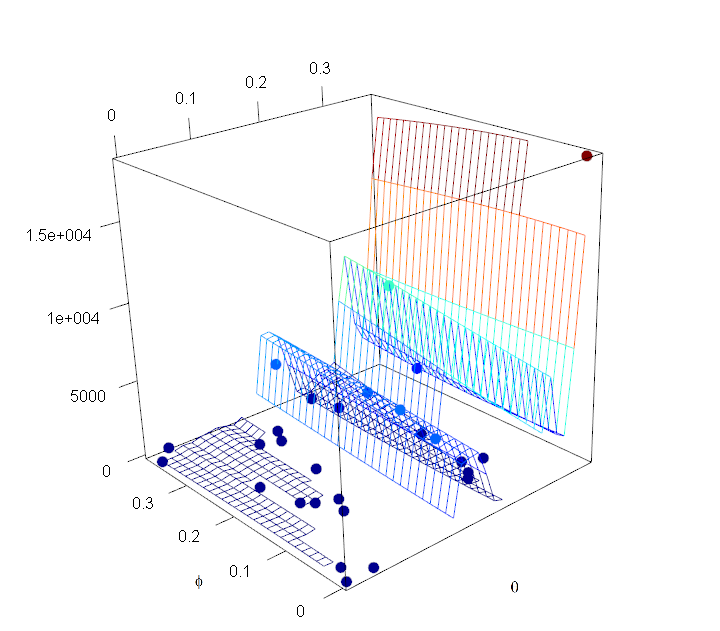
\includegraphics[width=7cm]{Figures/SensFinancialCapitalisation.png}
    \subcaption{Financial stranded assets}\label{Fig:SensFinStrand}
\end{minipage}
\vspace{0.2cm}
\caption{The effect of $\theta$ and $\phi$ on the low-carbon transition}\label{Fig:sensitivity}
\end{figure}



We will now study how climate market sentiments and limited information might modify the characteristics of the baseline low-carbon transition scenario. As explained in Section \ref{sec:exp}, we focus in particular on two parameters:
\begin{itemize}[noitemsep,nolistsep,leftmargin=*]
\item A parameter $\theta\in[0,1]$ representing climate financial apathy. The larger is $\theta$ the more will financial investors divert expected capital growth from the low-carbon to the high-carbon capital sector. This might be due to financial investors suffering from cognitive biases and professional incentives that lead them to prefer the status-quo. 
\item A parameter $\phi\in[0,1]$ representing investors’ blindness or, alternatively, the stickiness of their expectations. The larger is $\phi$ the stronger is be their tendency to stick to their previously expected capital values rather than adapting to the actual ones. This might be due to a limited circulation of data and information regarding low-carbon investment among financial professionals.
\end{itemize}

We follow the sampling method proposed by \citet{Salle2014}, for which sample points should be spread evenly throughout the parameter space. This is achieved using nearly-orthogonal Latin hypercube sampling \citep{Cioppa2002}\footnote{To that effect, we use the spreadsheet available in \citet{Sanchez2005}}. We carry out efficient sampling across the full parameter space, $(\theta,\phi) \in [0.0,1.0]$, gradually reducing the space to find the smallest area of the response surface that shows the essential behavior of the model. We find that the response variables in the space $(\theta,\phi) \in [0.0,0.4]$ yields the most meaningful results, and run 33 different models within this domain. The response surface can then be estimated at an arbitrary point using an adaptive weighting scheme (kriging) in which observed values closer to the point are given more weight. Kriging is a standard technique in geophysical sciences, and is explained in \citet{Salle2014}.

Figure \ref{Fig:sensitivity} shows the joint effect of the two parameters on the following set of relevant indicators\footnote{We abstract here from the scenarios in which no transition takes place (a total of six). This will be at the center of the analysis of Section \ref{sec:notrans}.}:
\begin{itemize}[noitemsep,nolistsep,leftmargin=*]
\item\emph{Exit period}: the number of periods that it takes for the high-carbon sector to exit the capital goods market.  
\item \emph{Output volatility}: an index of output volatility computed as the sum of the coefficient of variation of real output in each of the three sectors.
\item \emph{Physical stranded assets}: the quantity of existing capital stock owned by the high-carbon sector in the period before its default.
\item \emph{Financial stranded assets}: the market capitalization of the high-carbon capital sector in the period before its default\footnote{We use  lag values for both physical and financial stranded asset because the exit period might be triggered by three different conditions: non-positive profits in the high-carbon sector, non-positive output in the high-carbon sector or non-positive price of high-carbon equity.}.
\end{itemize}

The charts in Figure \ref{Fig:sensitivity} offer some interesting intuitions. Broadly speaking, the climate apathy parameter $\theta$ affecting expected sectoral growth rates seem to have much stronger effects than the blindness parameter $\phi$ for all indicators, with the exception of output volatility. The impact of the blindness parameter, for a given level of apathy, will be analyzed more in detail in Section \ref{sec:blindsim}. The larger is the value of $\theta$, the higher will be the number of periods it takes to fully achieve the transition (Figure \ref{Fig:SensExitPeriod}). Values of $\theta$ above 0.4 completely prevent the transition (results not shown here).

For the other indicators we observe strong non-linear behaviors, path dependencies and knife-edge dynamics. Non linear impacts of the apathy parameter seem to start for values larger than \(0.1\). This is confirmed by a sensitivity analysis (not shown) over the domain \((\theta,\phi)\in [0,0.1]\). The impact of financial apathy is larger for values around 0.2 than for values around 0.3. The analysis hereunder will show that this is due to stock effects and path dependency. In a nutshell, the portfolio specification leads to re-allocation between low-carbon and high-carbon sectors but also between capital and consumption sectors. This in turn triggers non-trivial impacts on investment, employment and hence total output but also to the relative size of each sector. Each of the two recession period (when the low-carbon emerges in the capital good market and when it enters the financial market) have more or less pronounced effect depending on these relative sectoral sizes. In certain cases, the economy settles into low capital stock regime (due to the growth function), implying an already deflated capital stock into the high-carbon sector, which leads to a smoother transition.

%%%%%%%%%%%%%%%%%%
\subsection{Failing the transition}
\label{sec:notrans}
%%%%%%%%%%%%%%%%%%
\begin{figure}[h!]
\begin{minipage}[b]{.5\linewidth}
\centering\large 
  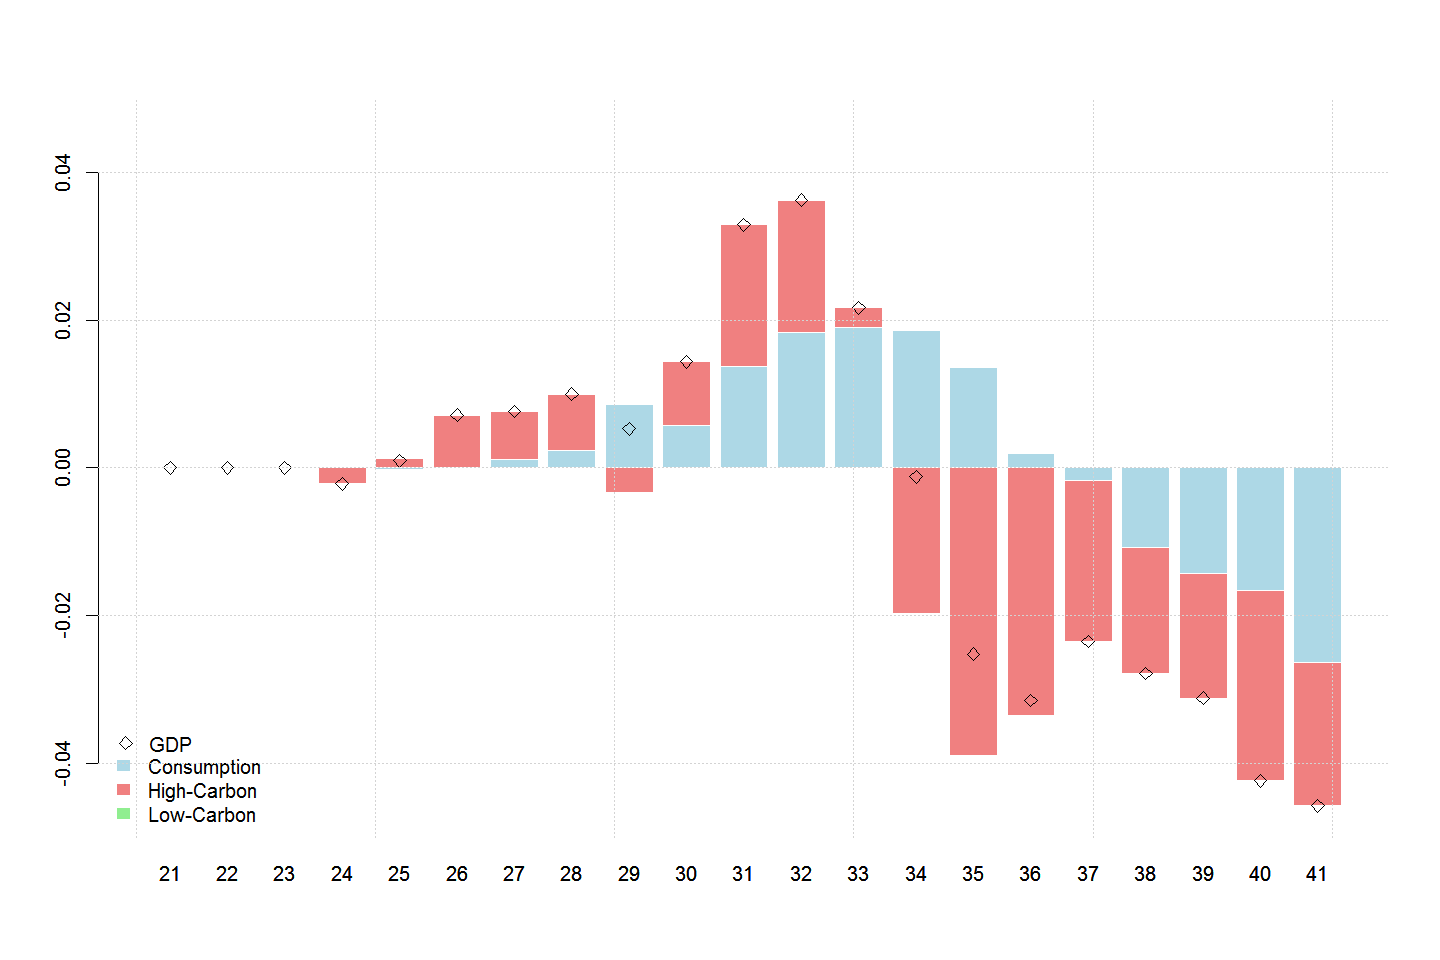
\includegraphics[width=7cm]{Figures/NoTransitionGDP.png}
  \subcaption{Sectoral output before the IPO}\label{Fig:NoTransGDP}
\end{minipage}%
  \quad \quad 
\begin{minipage}[b]{.5\linewidth}
\centering\large 
    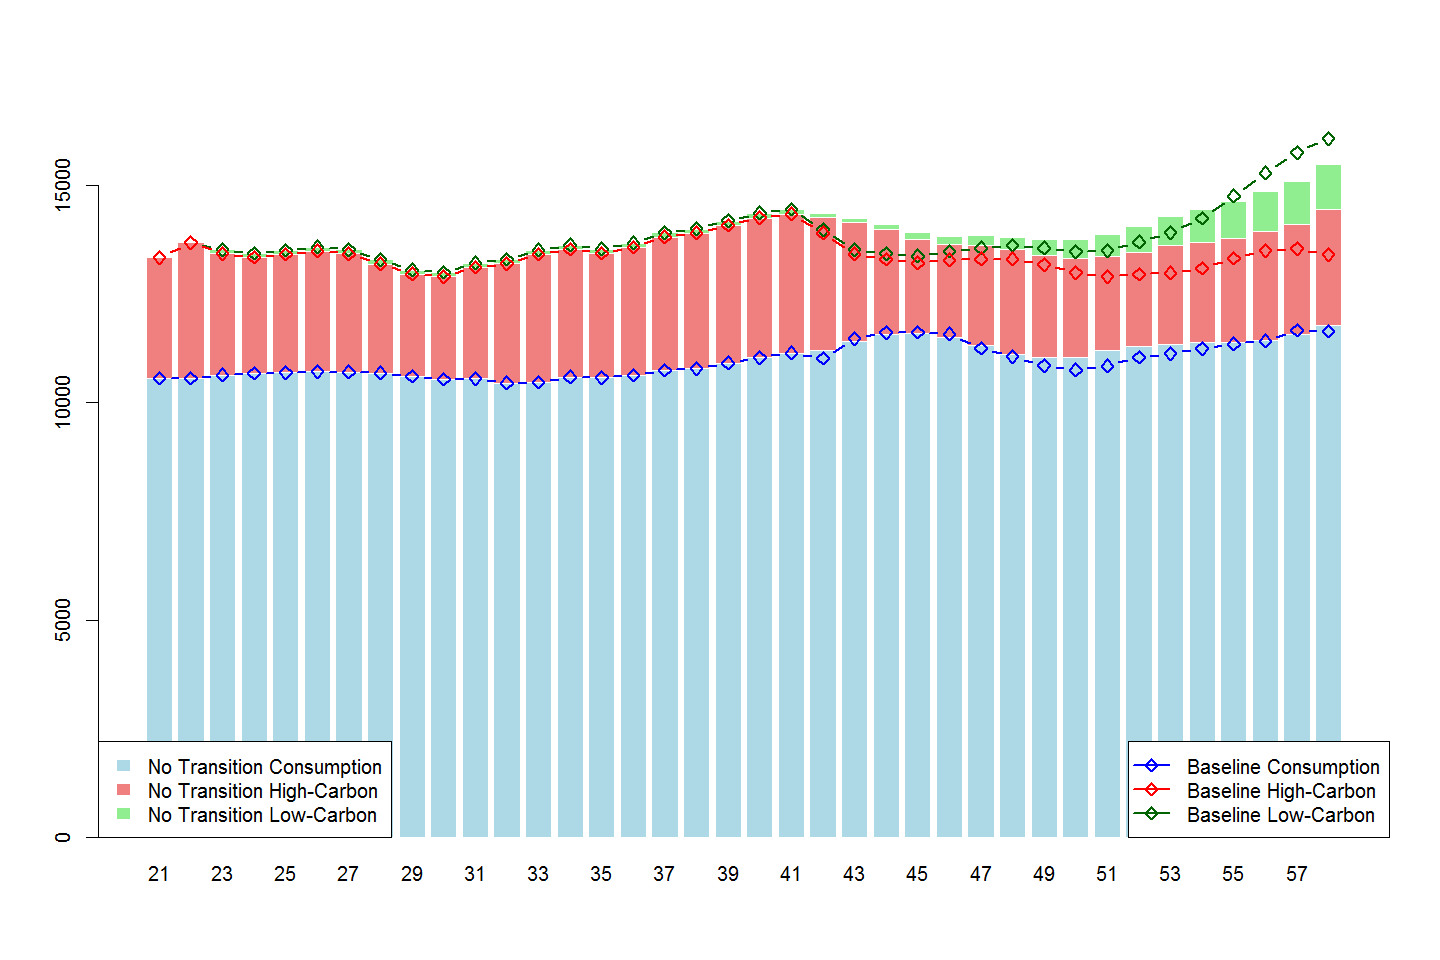
\includegraphics[width=7cm]{Figures/NoTransitionGDP2.png}
    \subcaption{Sectoral output after the IPO}\label{Fig:NoTransGDP2}
\end{minipage}
\vspace{0.2cm}
    \begin{minipage}[b]{.5\linewidth}
\centering\large 
   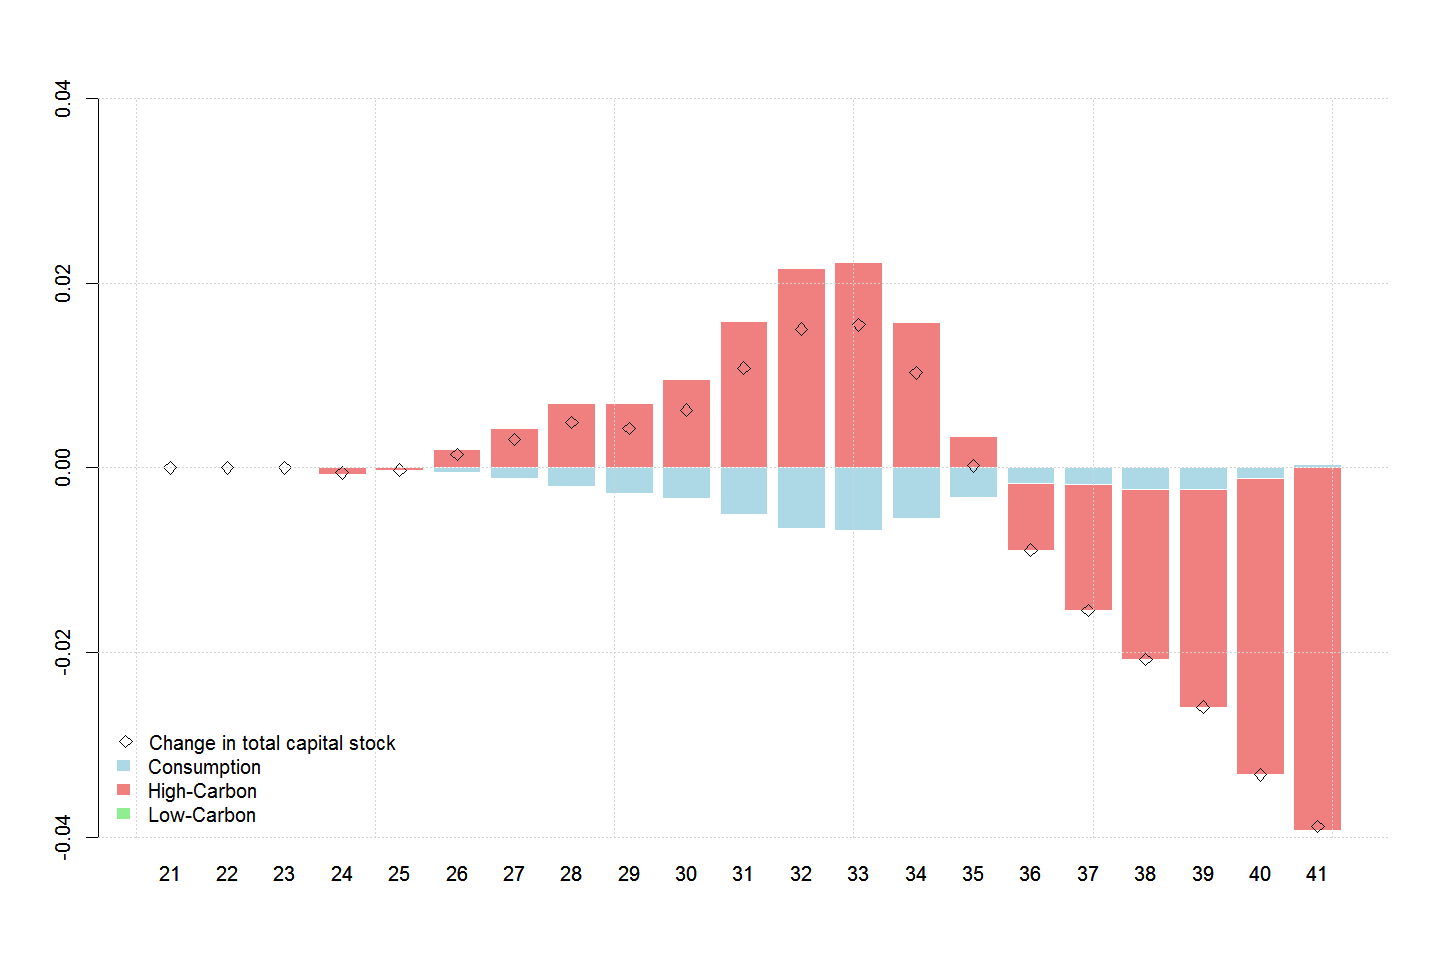
\includegraphics[width=7cm]{Figures/NoTransitionKStock.png}
    \subcaption{Capital stock}\label{Fig:NoTransK}
\end{minipage}
  \quad \quad 
    \begin{minipage}[b]{.5\linewidth}
\centering\large 
    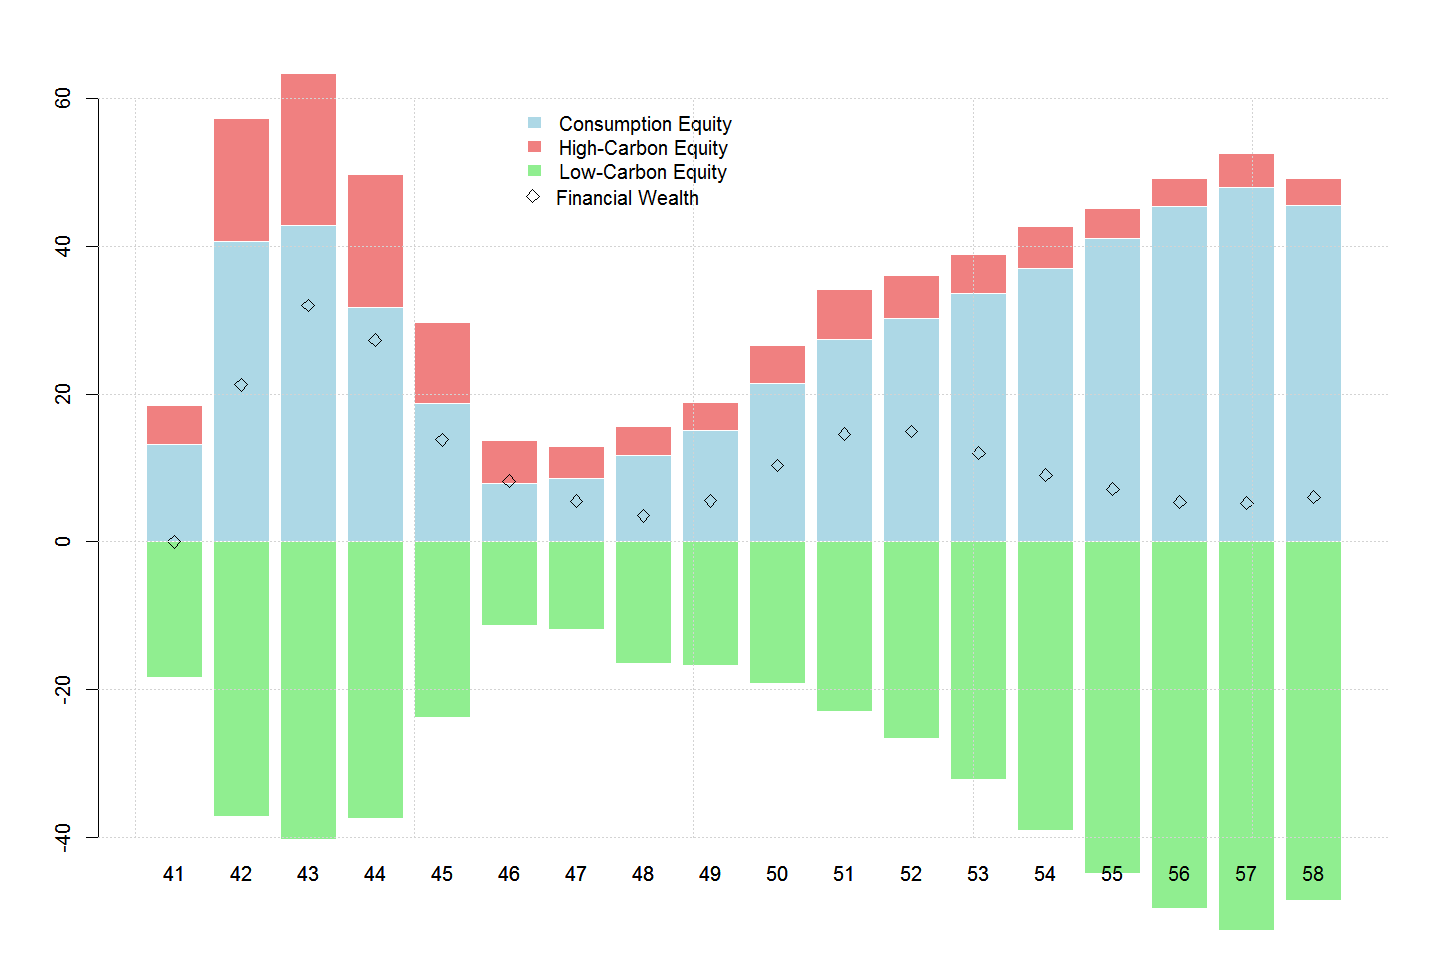
\includegraphics[width=7cm]{Figures/NoTransitionMarketCap.png}
    \subcaption{Market capitalisation}\label{Fig:NoTransMarketCap}
\end{minipage}
\vspace{0.2cm}
\caption{Comparison between the baseline scenario and scenario with no transition}\label{Fig:scen1}
\end{figure}

We next consider the conditions under which no transition occurs, using as an example a scenario with (\(\theta=0.35\) and \(\phi=0.175\)). As soon as the low-carbon sector enters the capital good market (period 20), it starts eating market share from the high-carbon sector, affecting the high-carbon sector growth rate. When financial investors are comparatively apathetic and blind to the changes, they give more weight to their belief about what the level of capital stock in the high-carbon sector ought to be than to what it actually is. They hence inflate the expected present value of the high-carbon capital stock, driving up the price of equity for the high-carbon sector and driving down the price of equity for the consumption sector. The presence of low-carbon capital affects financial markets indirectly, even though low-carbon assets are not yet available on financial markets. However, financial investors disregard the signals.

Overvaluation of high-carbon assets, combined with an initial demand for high-carbon capital from the low-carbon sector is stimulating. Overall, the impact is positive in terms of output, employment and labor income, a dynamic that is reinforced as the observed growth rates feed into investors' calculation of the present value of capital stocks. Higher labor income leads to increased consumption, reversing the initial negative impact on the consumption sector. Once this happens, the expected growth rate in the consumption sector overtakes that of the high-carbon capital sector, inducing a reallocation of wealth toward the consumption sector. This reallocation leads to slower (and eventually negative) growth in the high-carbon capital sector, with a corresponding decrease in output and employment. Note that this has no effect on the low-carbon sector dynamics which are identical as in the baseline scenario.

Greater blindness leaves the economy with a lower GDP and a lower capital stock in both the high-carbon and consumption sectors compared to the baseline. Lower capital stock in the aggregate leads to lower debt level (given the targeted leverage level), implying that money holding by households is lower, but this is partially compensated by a higher level of total market capitalisation.

The IPO, in period 40, of the low-carbon sector disrupts financial markets, as part of existing wealth currently invested in the high-carbon and consumption sectors is reallocated to the low-carbon sector. This leads to movements in equity prices, changes in Tobin's $q$, wealth loss, consumption effect and growth effects.

Blindness and apathy on the part of financial investors lead to some transfer of low-carbon growth toward the high-carbon capital good sector, leading to a much smaller shock (20\% lower) to both the high-carbon and consumption sectors. Indeed, as the expected present value of the low-carbon sector decreases, leading to an increase of the high-carbon sector, the expected present value of the consumption sector's capital stock remains proportionally higher. This implies higher financial wealth compared to the baseline and thus higher consumption, reflected in a milder recession after the IPO.

In summary, the combination of portfolio re-allocation and lower levels of GDP leads, on the one hand, to slower growth of the low-carbon sector in the non-transition scenario than in the baseline case. On the other hand, the high-carbon and consumption sectors grow much faster.

%%%%%%%%%%%%%%%%%%
\subsection{The impact of climate blindness}
\label{sec:blindsim}
%%%%%%%%%%%%%%%%%%

\begin{figure}[h!]
\begin{minipage}[b]{.5\linewidth}
\centering\large 
  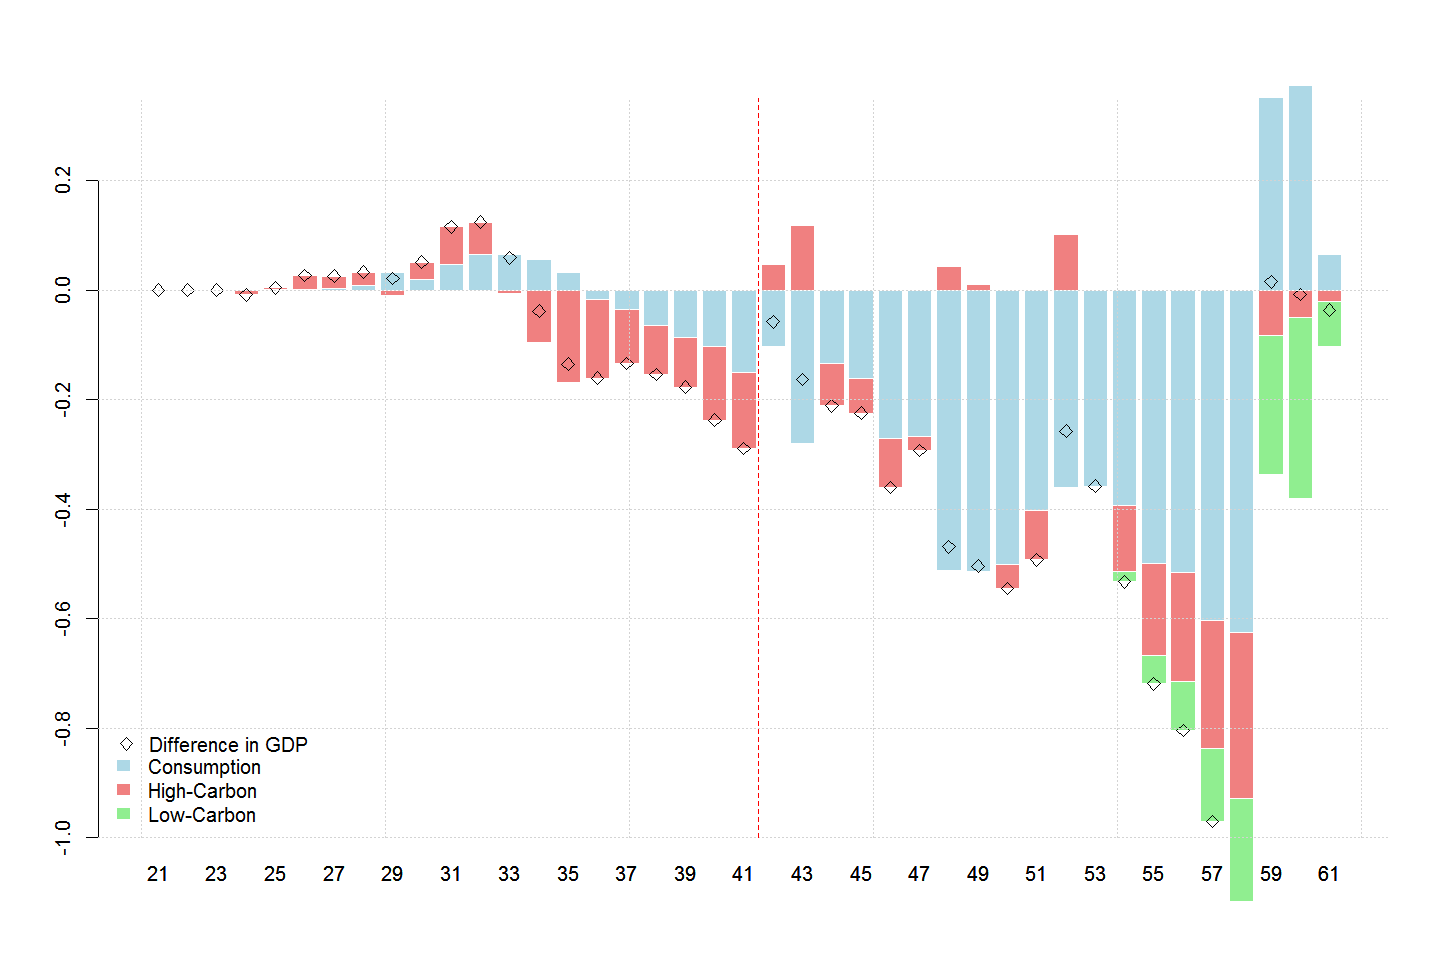
\includegraphics[width=7cm]{Figures/PhiGDP.png}
  \subcaption{Output}\label{Fig:PhiGDP}
\end{minipage}%
  \quad \quad 
\begin{minipage}[b]{.5\linewidth}
\centering\large 
   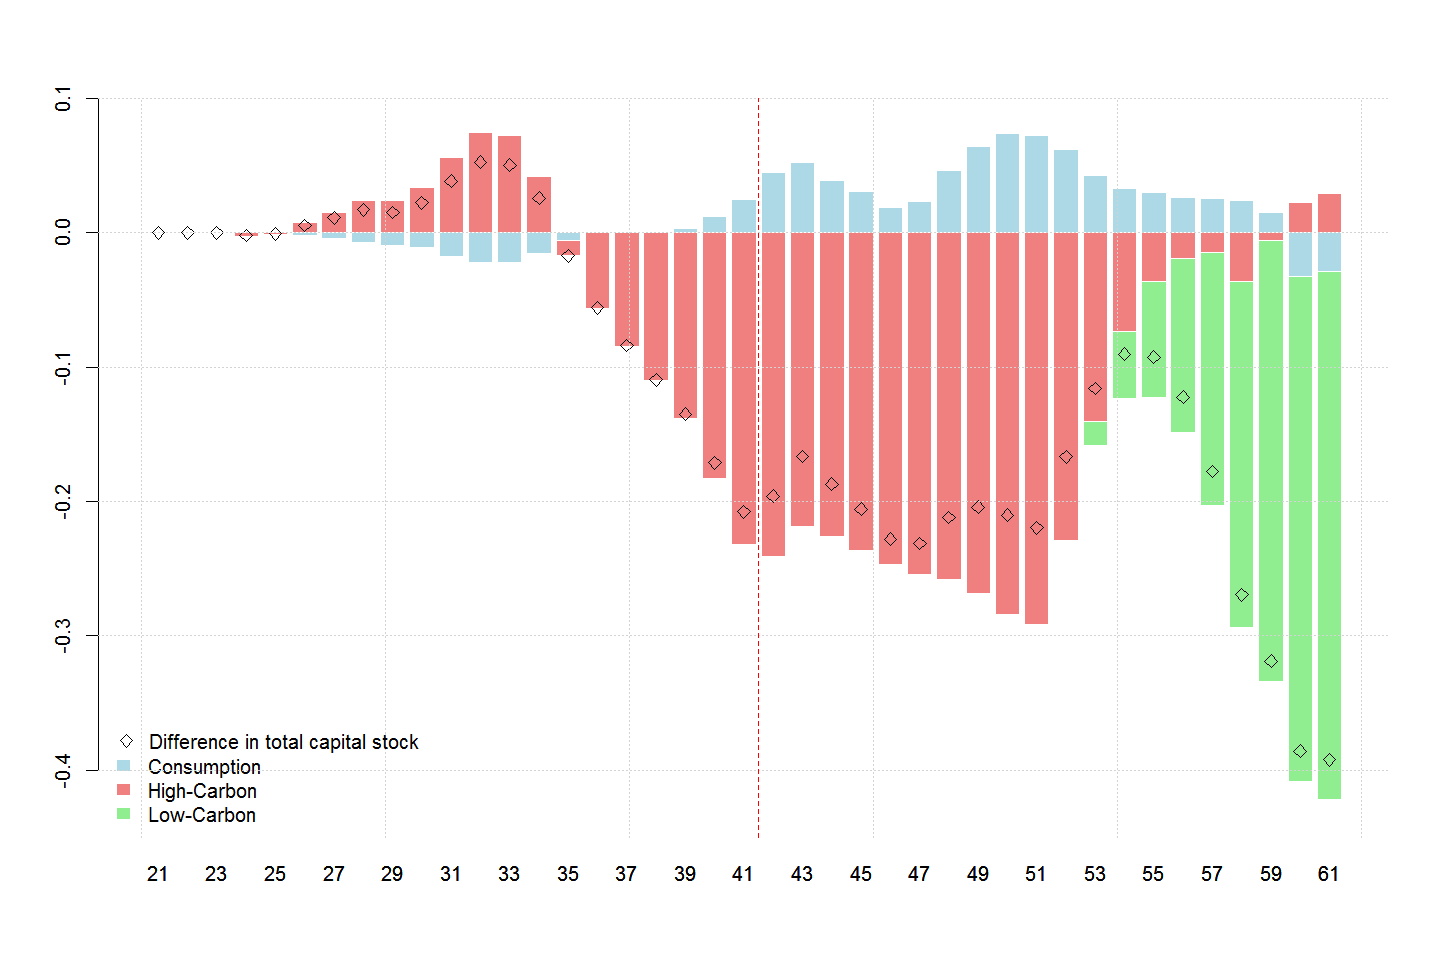
\includegraphics[width=7cm]{Figures/PhiCapStock.png}
    \subcaption{Capital stock}\label{Fig:PhiCapStock}
\end{minipage}
\vspace{0.2cm}
    \begin{minipage}[b]{.5\linewidth}
\centering\large 
    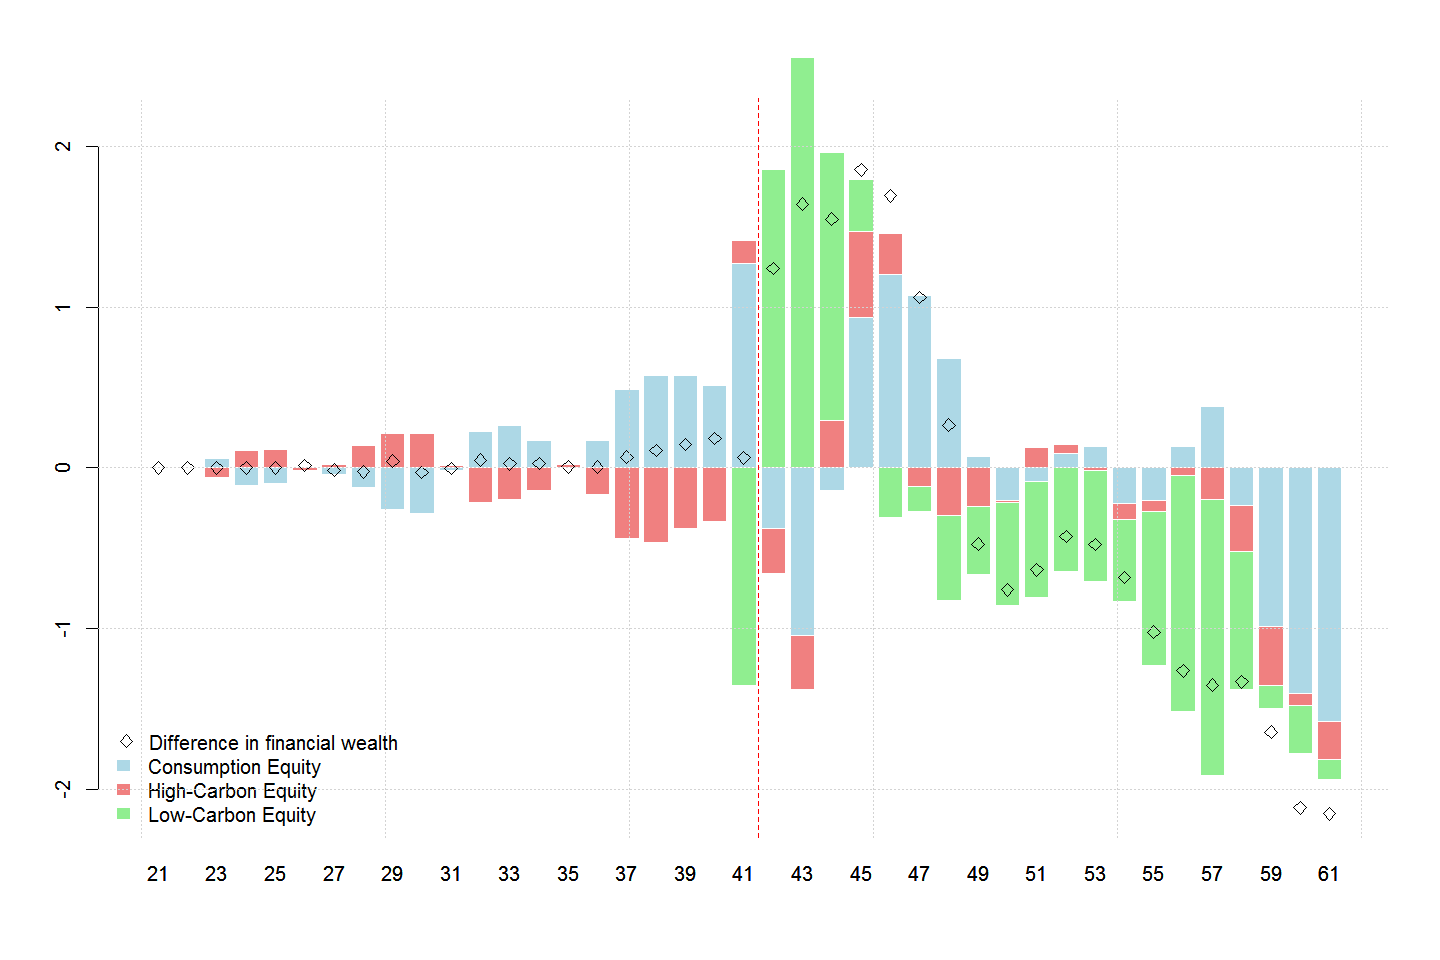
\includegraphics[width=7cm]{Figures/PhiMarketCap.png}
    \subcaption{Market Capitalization}\label{Fig:PhiMarketCap}
\end{minipage}
  \quad \quad 
    \begin{minipage}[b]{.5\linewidth}
\centering\large 
    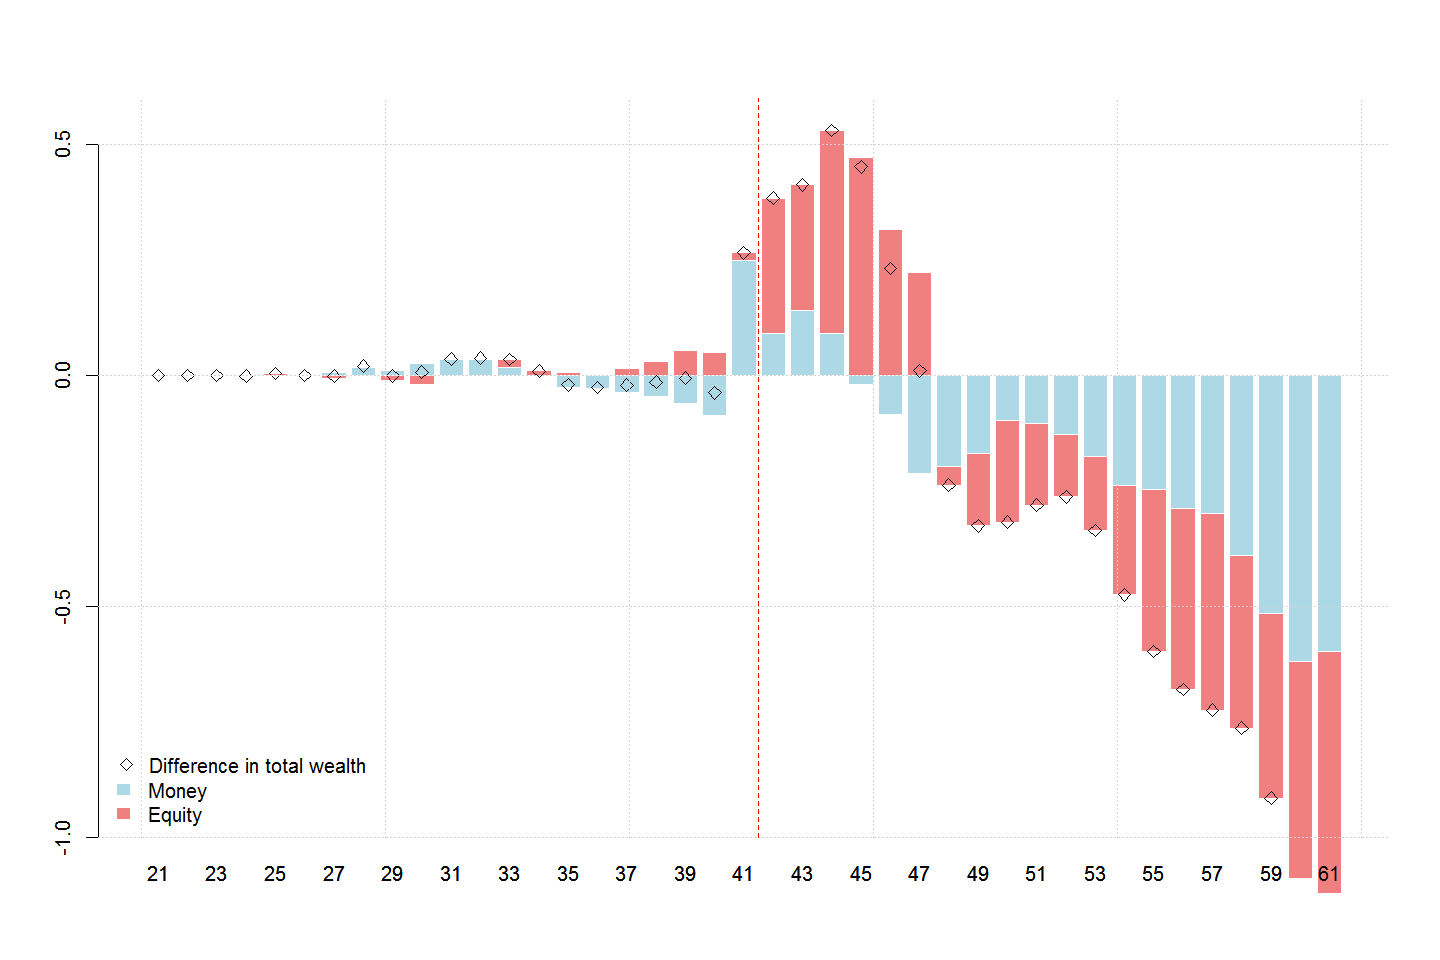
\includegraphics[width=7cm]{Figures/PhiWealth.png}
    \subcaption{Wealth}\label{Fig:PhiWealth}
\end{minipage}
\vspace{0.2cm}
\caption{Comparison between scenarios with two different levels of blindness}\label{Fig:scen2}
\end{figure}

As explained in section~\ref{sec:SensAnal}, the effect of the apathy parameters dominates most of the dynamics of the transition, and particularly the length of the transition and the quantity of real and financial stranded assets. We now turn to the case of understanding the effect of different levels of blindness  but identical apathy. To do so we run a different domain exploration based on three values for the apathy parameter ($\theta \in \left(0,0.1,0.2\right)$) and a complete domain sweep for the blindness parameter ($\phi \in \left(0,0.1,0.2,...,0.9,1\right)$). We observe that for low values of apathy, the blindness effect has little impact, except on the output volatility indicators (see Figure~\ref{Fig:SensOutputVol}). However, when apathy is larger ($\theta=0.2$), blindness has more significant impacts. We thus compare two scenarios; one ($\phi=1$) displaying a transition with a relatively smaller recession when the high-carbon sector defaults, and one ($\phi=0.3$) displaying a transition with a larger recession. Note that the transition takes place in either cases.

As already explained, the entry of the low-carbon sector leads to a re-allocation of financial assets which have an impact on the growth rate of consumption and high-carbon sectors. However, higher blindness leads to further overvaluation of the high-carbon equity price (around 0.3\% in the first period) and undervaluation of the consumption equity price (around 0.1\%). The difference in blindness thus leads to a variation of the business cycle emerging out of the low-carbon firms entry on the capital marker. The difference in portfolio allocation due to different expected present value feed back into employment, consumption, and in the consumption sector capital stock. This reverses the portfolio allocation towards the consumption sector and leads to a decrease in the high-carbon investment strategy. In the end, blinder financial investor actually smooth the business cycle by discounting more of the green capital stock and thus over-valuing the high-carbon capital stock. This
leads to less abrupt fluctuation. This is shown in Figure~\ref{Fig:PhiGDP} displaying the difference in GDP component between the two transitions (less blind values minus blinder values) as a percentage of current GDP. We can see that blinder financial investor leads to much smaller GDP fluctuation, of the order of magnitude of up to 1\% of GDP.

Again, the effect on the capital stock are striking, more blindness leaves the economy with a lower capital stock in the brown sector and a slightly higher capital stock in the consumption sector. Overall, the economy has a lower stock of capital (see Figure~\ref{Fig:PhiCapStock}).

Lower capital stock in the aggregate leads to lower debt level (given the targeted leverage level), implying that money holding by households is lower, but this is partially compensated by a higher level of total market capitalization (see Figure~\ref{Fig:PhiWealth}).

Once the green sector enters the financial market, most of the dynamics are dominated by the portfolio re-allocation process and its feed-back to real dimensions such as growth, employment, consumption and investment. The fact that the brown capital sector was already smaller means that the shock of the green IPO is relatively lower, leading to a phase where total financial wealth is not as depressed as in the less-blind scenario. However, this is only transitory as soon the reality of real capital stock levels drags down the market capitalization of all firms into level lower in the blinder case.

On the flow side, the situation pre-IPO remain the norm, i.e. lower consumption and overall lower investment in brown capital. This even leads to lower low-carbon investment towards the end of the transition.

On the stock space, the level of capital stock remains slightly higher in the blinder scenario while the large gap in high-carbon capital stock slowly disappears (due to lower decrease in capital stock than in the less-blind scenario). The observed decrease in green investment translates in a lower level of low-carbon capital stock.

When the high-carbon sector defaults, the economy is thus in a situation where there is less capital stock (11\% difference), less debt (7\% difference) and a lower market capitalization (3\% difference) in the traditional capital sector. This imply that the disappearance of that sector is less of a shock and hence allow for a quicker recovery afterward. 

The interesting conclusion from this scenario analysis is that, as for the no-transition scenario analysis, pre-IPO dynamics explain most of the reason for a difference in the amplitude of shock due to the default of the brown sector. The blindness parameter affects at first the consumption sector which launch the economy to a path including a lower level of GDP and a lower level of stocks.

%%%%%%%%%%%%%%%%%%
%%%%%%%%%%%%%%%%%%
\section{Conclusions}
\label{sec:concl}
%%%%%%%%%%%%%%%%%%
%%%%%%%%%%%%%%%%%%

The perceptions and expectations that financial investors develop around the likelihood and speed of the transition to a low-carbon economy might play a crucial role in shaping its dynamics. A combination of behavioral biases and imperfect knowledge might lead investors to under-estimate the potential for development of low-carbon sectors and allocate their financial wealth disproportionately into high-carbon assets. Prevalent climate sentiments in the financial industry might delay or possibly prevent the shift to clean capital stocks, even when the latter are economically more convenient. 

In this paper we have presented a novel modelling framework capable of grasping some key features of the multiple links connecting financial investment decisions, macroeconomic dynamics and the large-scale process of shifting to low-carbon forms of capital stock. The model includes two capital goods – high-carbon and low-carbon – and financial investors allocating their portfolio across the equities of the productive sectors according to both long-term expectations on the development of the sectors and short-term considerations linked to return rates. 

Our baseline scenario with `unbiased expectations' shows how the emergence of a new, innovative, carbon-free capital produces large macroeconomic and financial effects. These are particularly pronounced after the high-carbon capital sector is driven out of business. We then investigate how apathetic expectations and limited information might affect the transition dynamics. We show that higher levels of climate apathy extend the length of the transition period and increase the amount of both physical and financial stranded assets. We also show how the the climate blindness parameter, while having little effect when combined with low levels of apathy, produces non-trivial impacts when in combination with higher level of apathy.

While offering a novel perspective on how market sentiments affect the low-carbon transition, the present study is not free of limitations. For instance, as explained in Section \ref{sec:concept}, the specific research questions addressed here lead us to abstract from the market and policy conditions required for the transition to take place. While we assume the low-carbon capital to be economically convenient for firms investing in physical capital, this is still not the case in the real world. A number of regulatory, fiscal and monetary policies might be needed in order for this to actually happen, with further macroeconomic and financial repercussions. This will be the focus in the prosecution of our research.  

However, we are already able to draw some policy implications from the current analysis. For instance, it is clear that reassuring financial investors of the long-term expansion prospects of low-carbon activities (e.g. power generation from renewable sources, electric mobility, pollution-free industrial processes) is of paramount importance. For this to happen, stability and credibility of environmental fiscal policies and regulations is essential, as well as a science-based policy-making process.  Widespread information is also crucial; for instance, \citet{TCFD2016} argues for a more comprehensive and standardised disclosure of climate-related risks by private companies that might help investors to have a clearer perception of the diffusion of high-carbon and low-carbon technologies. The diffusion of standardised financial instruments like green bonds is another common suggestion \citep{CBI2016}. Public institutions could also intervene by de-risking low-carbon investment, introducing prudential regulation or incentivizing better performance assessment methods \citep{UNEPInquiry2015}.


%%%%%%%%%%%%%%%%%%%%%%%%%%%%%%%%%%%%%%%%%
\newpage
\appendix
%%%%%%%%%%%%%%%%%%%%%%%%%%%%%%%%%%%%%%%%%


%\section{List of variables and parameters}


%\newpage
\bibliographystyle{chicago}
\bibliography{ClimateFinBubbles}


\begin{comment}

CEMETERY 

%%%%%%%%%%%%%%%%%%%%%%%%%%%%%%%%%%%%%%%%%%%%%%%%%%%%%%%%

Financial investors also form expectations regarding the future growth of the sectors, which then inform their wealth allocation choices. The `unbiased' expectations, denoted by the $BAU$ superscript, are a function of observed average sectoral capital growth over the last four periods. 

\begin{gather}
\hat{k}^{BAU}_{c} = \frac{1}{4}\sum_{t=0}^3 \frac{k_{h,c} + k_{l,c} - k_{h,c,-1} - k_{l,c,-1}}{k_{h,c,-1} + k_{l,c,-1}}\\
\hat{k}^{BAU} = \frac{1}{4}\sum_{t=0}^3 \frac{k_{h,h} + k_{h,l} + k_{l,l} - k_{h,h,-1} - k_{h,l,-1} - k_{l,l,-1}}{k_{h,h,-1} + k_{h,l,-1} + k_{l,l,-1}}\\
\hat{k}^{BAU}_{l} = \frac{1}{4}\sum_{t=0}^3 \frac{k_{h,l} + k_{l,l} - k_{h,l,-1} - i_{l,l,-1}}{k_{h,l,-1} + i_{l,l,-1}}\\
\hat{k}^{BAU}_{h} = \frac{1}{4}\sum_{t=0}^3 \frac{k_{h,h} - k_{h,h,-1}}{k_{h,h,-1} }
\end{gather}


However, as argued in Section \ref{sec:intro}, financial investors might have `apathetic' expectations regarding the development of the low-carbon capital sector. We thus allow investors to `reallocate' part of their expected growth in capital stocks from the low-carbon to the high-carbon sector depending on a `climate apathy' parameter $\theta$, while keeping the total growth of the capital sector $\hat{k}^{BAU}$ constant. For simplicity, we assume expected growth rates of the consumption sector $\hat{k}^{BAU}_{c}$ to remain `unbiased'.

\begin{gather}
\hat{k}_{l}^e = \theta \frac{\hat{k}^{BAU}- \sigma_h \hat{k}^{BAU}_h}{1-\sigma_h}\\
\hat{k}_{h}^e = \frac{\hat{k}^{BAU}-(1-\sigma_h) \hat{k}^e_{l}}{\sigma_h}\\
\hat{k}_{c}^e = \hat{k}^{BAU}_{c}
\end{gather}

where $\sigma_h = \dfrac{k_{h,h}}{k_{h,h} + k_{h,l} + k_{l,l}}$ is the share of high-carbon capital over total capital.


%%%%%%%%%%%%%%%%%%%%%%%%%%%%%%%%%%%%%%%%%%%%%%%%%%%%%%%%

\begin{figure}
\centering
\begin{subfigure}{.5\textwidth}
  \centering
  \includegraphics[width=.9\linewidth]{Figures/DeltaOutput.png}
  \caption{A subfigure}
  \label{fig:sub1}
\end{subfigure}%
\begin{subfigure}{.5\textwidth}
  \centering
  \includegraphics[width=.9\linewidth]{Figures/EquityPrice.png}
  \caption{A subfigure}
  \label{fig:sub2}
\end{subfigure}
\caption{A figure with two subfigures}
\label{fig:test}
\end{figure}

\begin{figure}[]
\begin{minipage}[b]{0.49\linewidth}
\centering
a - Nominal sectoral GDP 
\includegraphics[width=1\textwidth]{Figures/DeltaOutput.png}
\end{minipage}
\hspace{0.1cm}
\begin{minipage}[b]{0.49\linewidth}
\centering
b - Sectoral equity price
\includegraphics[width=1\textwidth]{Figures/equityPrice.png}
\end{minipage}
\caption{Baseline scenario TO BE REPLACED WITH UPDATED PICTURES}
\label{fig:base}
\end{figure}

%%%%%%%%%%%%%%%%%%%%%%%%%%%%%%%%%%%%%%%%%%%%%%%%%%%%%%%%

We assume two types of external finance in the model: bank credit and emission of new equity. [EKB START] We assume that firms compare the realized return on capital to a target, $r_x^T$, where the realized return is the spread between previous period capital gains, $cg_{x,-1}$, and the interest due on loans, $r_{lx}$. The share $\Psi_x$ of excess investment funded by new equity in sector $x$ is assumed to rise, follow a sigmoid curve that increases as the realized return exceeds the target:[EKB END]
\begin{align}
\Psi_x = \frac{1}{1 + e^{\psi_x\left(r_x^T - cg_{x,-1} - r_{lx}\right)}}
\end{align}
where, $r_x^T$ is the target return on capital, $cg_{x,-1}$ are real capital gains from the previous period, $r_{lx}$ is the interest rate on loans, and $\psi_x$ is a calibration parameter [WHY? EXPLAIN RATIONALE][EKB SEE ABOVE].

New equity issue $e^s_x$ in sector $x$ is determined by the nominal value of the needed finance and the previous period value of the equity. Newly emitted equities are added to the existing stock to determine the total number of equities in a sector.
\begin{gather}
e^s_x = \dfrac{\Psi_x I_{fx}}{p_{e,x,-1}} \\
e_x = e_{x,-1} + e^s_x
\end{gather}

The remaining portion of excess investment ($I_x-F_x-e_x^s p_{x,e}$) is financed through bank credit. 


\end{comment}






\end{document}











